% concatenated from adjoint-transport-en.tex
% Build from /home/momota1029/doc with:
% latexmk-diff-head writing/adjoint-transport/adjoint-transport-en
\documentclass{amsart}

\usepackage{amsmath,amssymb,amsthm,mathtools}
\usepackage{enumitem}
\usepackage{array,longtable}
\usepackage{ifpdf}
\ifpdf
\else
\def\pgfsysdriver{pgfsys-dvipdfmx.def}
\fi
\usepackage{tikz-cd}
\ifpdf
\usepackage[hidelinks]{hyperref}
\else
\usepackage[dvipdfmx,hidelinks]{hyperref}
\fi
\usepackage{cleveref}

\theoremstyle{plain}
\newtheorem{theorem}{Theorem}[section]
\newtheorem{proposition}[theorem]{Proposition}
\newtheorem{lemma}[theorem]{Lemma}
\newtheorem{corollary}[theorem]{Corollary}
\crefname{theorem}{Theorem}{Theorems}
\crefname{proposition}{Proposition}{Propositions}
\crefname{lemma}{Lemma}{Lemmas}
\crefname{corollary}{Corollary}{Corollaries}

\theoremstyle{definition}
\newtheorem{definition}[theorem]{Definition}
\newtheorem*{definition*}{Definition}
\crefname{definition}{Definition}{Definitions}

\theoremstyle{remark}
\newtheorem{remark}[theorem]{Remark}
\crefname{remark}{Remark}{Remarks}
\crefname{section}{Section}{Sections}
\crefname{equation}{Equation}{Equations}
\crefname{figure}{Figure}{Figures}

\newcommand{\R}{\mathbb{R}}
\newcommand{\D}{\mathcal{D}}
\newcommand{\X}{\mathcal{X}}
\newcommand{\Xp}{\mathcal{X}^{+}}
\newcommand{\M}{\mathcal{M}}
\newcommand{\DM}{\mathcal{DM}}
\renewcommand{\L}{\mathcal{L}}
\newcommand{\TB}{\mathcal{TB}}
\newcommand{\Lup}{\operatorname{Lip}^{+}_{1}(\R)}
\newcommand{\lipplus}{\operatorname{Lip}^{+}_{1}}
\DeclareMathOperator{\lipone}{Lip_1}
\DeclareMathOperator{\dis}{dis}
\DeclareMathOperator{\supp}{supp}
\DeclareMathOperator{\pr}{pr}
\newcommand{\dconc}{d_{\operatorname{conc}}}
\newcommand{\dpr}{d_{\operatorname{P}}}
\newcommand{\kf}{d_{\operatorname{KF}}}
\newcommand{\dinf}[1]{d^{#1}_{\infty}}
\newcommand{\haus}[1]{\left(#1\right)_H}
\newcommand{\Tplan}{\mathcal{T}}

\title[Pyramidal Compactification via Adjoint Transport]{Pyramidal Compactification of Asymmetric Metric Measure Spaces via Adjoint Transport}
\author{Shigeaki Yokota}
\date{}
\keywords{pyramidal compactification, quasi-metric measure space, asymmetric metric measure space, adjoint transport, box distance, pyramid}
\subjclass[2020]{Primary 53C23; Secondary 54E35, 28A33}

\begin{document}

\begin{abstract}
A quasi-metric measure space (qm-space) is a set with a directed distance whose symmetrization is a complete separable metric, together with a Borel probability measure of full support. Motivated by the problem of determining the pyramid limits of beta measures on forward Funk balls, we construct a compact metric space of pyramids of qm-spaces. The associated-pyramid map from the concentration-distance space of qm-spaces into this compact space is a $1$-Lipschitz topological embedding with dense image. As a secondary result, we prove that the box-distance space of qm-spaces is complete and separable.
\end{abstract}

\maketitle

\section{Introduction}
\label{sec:introduction}
To interpret the L\'evy--Milman concentration-of-measure phenomenon in high-dimensional spaces as geometric convergence, Gromov developed the concentration theory of mm-spaces. A triple $(X,d_X,\mu_X)$ is an \emph{mm-space} if $(X,d_X)$ is a complete separable metric space and $\mu_X$ is a Borel probability measure of full support. We write $\X$ for the set of isomorphism classes of mm-spaces. The concentration topology is strictly weaker than the measured Gromov--Hausdorff topology. For a fibration whose fibers form a L\'evy family, it collapses the fibers to points while retaining the base as the limit, and thus allows convergence and limits to be studied for sequences of unbounded dimension \cite[Introduction]{shioya2016mmg}. Gromov introduced the observable distance that measures this convergence and the box distance, whose topology is strictly finer \cite{gromov2007met}. We denote these distances by $\dconc$ and $\Box$, respectively.

For mm-spaces $X$ and $Y$, say that $X$ dominates $Y$ if there exists a measure-preserving $1$-Lipschitz map from $X$ to $Y$. A \emph{pyramid} is a nonempty subset of $\X$ that is downward closed under this relation, closed with respect to $\Box$, and contains a common upper bound for each pair of its elements. We write $\Pi$ for the set of all pyramids. For each $X\in\X$,
\[\mathcal P_{\mathrm{mm}}(X)\coloneqq\{Y\in\X\mid X\text{ dominates }Y\}\]
is a pyramid and defines the associated-pyramid map introduced by Gromov,
\[\iota\colon\X\longrightarrow\Pi,\qquad X\longmapsto\mathcal P_{\mathrm{mm}}(X)\]
\cite{gromov2007met,esaki-kazukawa-mitsuishi2024cones}. Shioya metrized pyramid weak convergence and made $\Pi$ a compact metric space \cite[Definition~4.5 and Theorem~4.6]{shioya2022sugaku}. We denote this metric by $d_\Pi$. This compactification captures measure concentration while retaining both distance and measure, but its use of symmetric distances does not preserve the order of directed endpoints.

The forward Funk beta model is a concrete case in which this limitation matters. For $n\geq1$ and $\beta>0$, let $\mathbb B^n\coloneqq\{x\in\mathbb R^n\mid |x|<1\}$ be the Euclidean unit ball, and write $dx$ for Lebesgue measure on $\mathbb R^n$. Define the beta probability measure on $\mathbb B^n$ by
\[d\mu_{n,\beta}(x)\coloneqq\frac{\Gamma(n/2+\beta)}{\pi^{n/2}\Gamma(\beta)}(1-|x|^2)^{\beta-1}\,dx,\]
and equip the ball with the forward Funk distance $d_{\mathrm F}$. The Klein distance $d_{\mathrm K}$ and the potential $\phi(x)\coloneqq-\frac12\log(1-|x|^2)$ satisfy, for all $x,y\in\mathbb B^n$,
\[d_{\mathrm F}(x,y)=d_{\mathrm K}(x,y)+\phi(y)-\phi(x).\]
Its symmetrization is
\[d_{\mathrm F}^{\mathrm s}(x,y)=d_{\mathrm K}(x,y)+|\phi(y)-\phi(x)|,\]
which replaces the signed endpoint increment by its absolute value. Indeed, for $0<r<1$ and a unit vector $\theta\in\mathbb R^n$,
\[d_{\mathrm F}(0,r\theta)=-\log(1-r)\longrightarrow+\infty,\qquad d_{\mathrm F}(r\theta,0)=\log(1+r)\leq\log2.\]
Thus symmetrization cannot distinguish which endpoint carries the potential. For a positive sequence $(\beta_n)$, the concrete three-phase limits of this model are proved in the sister paper \cite{finsler-poincare-beta-balls}. That paper depends mathematically on the theory of the present paper, while the present paper uses none of its results.

The fixed statements from the two upstream papers on geometric data sets used here, together with their roles and first-use locations, are recorded in \Cref{sec:upstream-dependencies}.

To preserve this endpoint order, a triple $(X,d_X,\mu_X)$ is called a \emph{quasi-metric measure space (qm-space)} if $d_X$ is a directed distance whose symmetrization is defined, for all $x,y\in X$, by
\[d_X^{\mathrm s}(x,y)\coloneqq\max\{d_X(x,y),d_X(y,x)\}\]
and is a complete separable metric, and if $\mu_X$ is a Borel probability measure of full support. We write $\Xp$ for the set of isomorphism classes of qm-spaces. A measure-preserving map $u\colon X\to Y$ between qm-spaces is \emph{$1$-Lipschitz} if
every pair $x,x'\in X$ satisfies
\[d_Y(u(x),u(x'))\leq d_X(x,x').\]
We write $Y\preceq X$ when such a map exists, and set
\[\mathcal P(X)\coloneqq\{Y\in\Xp\mid Y\preceq X\}.\]
Let $X$ be the three-point qm-space on $\{a,b,c\}$ shown in \Cref{fig:three-point-directed-obstruction}. After symmetrization, its lower set contains the two-point mm-space with masses $0.6,0.4$ and distance $1$, whereas $\mathcal P(X)$ excludes the corresponding qm-space because its reverse distance exceeds $0.1$. This is the smallest finite example of the information lost by classical symmetrization.

\begin{figure}[t]
\centering
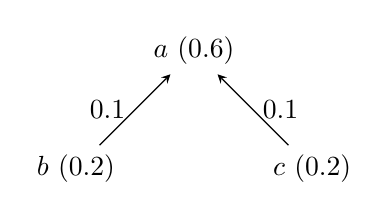
\begin{tikzpicture}[>=stealth]
\node (a) at (0,1.5) {$a\ (0.6)$};
\node (b) at (-1.5,0) {$b\ (0.2)$};
\node (c) at (1.5,0) {$c\ (0.2)$};
\draw[->] (b) -- node[left] {$0.1$} (a);
\draw[->] (c) -- node[right] {$0.1$} (a);
\end{tikzpicture}
\caption{The three-point qm-space $X$. The displayed arrows give $d_X(b,a)=d_X(c,a)=0.1$. Every other nonzero directed distance is $2$.}
\label{fig:three-point-directed-obstruction}
\end{figure}

On $\Xp$, we use $\dconc$ for the observable distance determined by one-sided observables and $\Box$ for the directed version of the box distance. By \cite[Proposition~5.8]{gds1}, one has $\dconc\leq\Box$. A subset of $\Xp$ is a pyramid if it is nonempty, downward closed under $\preceq$, closed with respect to $\Box$, and contains a common upper bound for each pair of its elements. We write $\Pi^+$ for the set of all such pyramids. Does the same compactification hold while preserving the order of directed endpoints?

\begin{theorem}[Pyramidal compactification of qm-spaces]
\label{thm:intro-qm-pyramidal-compactification}
For every $X\in\Xp$, the lower set $\mathcal P(X)$ belongs to $\Pi^+$. There exists a metric $d_{\Pi}^{\M}$ on $\Pi^+$ with the following properties.
\begin{enumerate}[label=\textup{(\roman*)}]
\item The metric space $(\Pi^+,d_{\Pi}^{\M})$ is compact.
\item For all $X,Y\in\Xp$,
\[d_{\Pi}^{\M}(\mathcal P(X),\mathcal P(Y))\leq\dconc(X,Y),\]
and $X\mapsto\mathcal P(X)$ is a topological embedding of $(\Xp,\dconc)$ into $(\Pi^+,d_{\Pi}^{\M})$.
\item The image $\{\mathcal P(X)\mid X\in\Xp\}$ is dense in $(\Pi^+,d_{\Pi}^{\M})$.
\end{enumerate}
\end{theorem}

\Cref{tab:introduction-overview} shows the correspondence between the four layers of the construction and the three conclusions of the main theorem.

\begin{table}[t]
\centering
\small
\setlength{\tabcolsep}{3pt}
\renewcommand{\arraystretch}{1.15}
\begin{tabular}{>{\raggedright\arraybackslash}p{0.16\textwidth}>{\raggedright\arraybackslash}p{0.20\textwidth}>{\raggedright\arraybackslash}p{0.25\textwidth}>{\raggedright\arraybackslash}p{0.27\textwidth}}
\hline
Layer & Input & Conclusion obtained & Role in the main theorem\\
\hline
Distance recovery & Ordered increments of one-sided observables & The directed distance and its symmetrization are recovered & Prevents loss of the directed object under representation\\
Box geometry & Observable families on coupled probability spaces & $(\Xp,\Box)$ is complete and separable & Supplies closedness and approximation for lower sets\\
Finite measurements & Bounded ordered observations & Pyramid weak convergence is decided and metrized & Turns transported convergence into the metric $d_{\Pi}^{\M}$\\
Pyramid compactification & Lower sets and the representation--reconstruction adjunction & Compactness, embedding, and density & Realizes the directed compactification\\
\hline
\end{tabular}
\caption{The four structural layers of the compactification.}
\label{tab:introduction-overview}
\end{table}

One-sided observables retain the order of an increment and thereby the two directed distances that symmetrization identifies. The representation--reconstruction adjunction transports the pyramid compactification to qm-spaces, together with its weak convergence and compactness.

The appendices give a categorical general theory of pyramid transport and ordered measurements that applies beyond qm-spaces.

\section*{Notation and standing conventions}

We write $\R$ for the real line, $\supp\mu$ for the support of a measure $\mu$, and $u_*\mu$ for the pushforward of $\mu$ by a measurable map $u$. Once a category of spaces or gd-sets has been introduced, the same symbol is also used for its set of isomorphism classes, and we do not distinguish notationally between an object and its isomorphism class.

For a distance or pseudodistance $d$ and a nonempty subset $A$, write
\[d(x,A)\coloneqq\inf_{a\in A}d(x,a),\]
and denote the Hausdorff distance or pseudodistance induced by $d$ on sets by $\haus{d}$. For real-valued Borel functions $h,k$ on a probability space $(W,\omega)$, set
\[\kf^\omega(h,k)\coloneqq\inf\{\varepsilon>0\mid\omega(|h-k|>\varepsilon)\leq\varepsilon\}.\]
This is the Ky Fan metric with respect to $\omega$.
For a measured space $X$ with distinguished probability measure $\mu_X$, we abbreviate $\kf^{\mu_X}$ to $\kf^X$.
We write $\dpr$ for the Prokhorov distance whenever the underlying metric is clear.

We write $\Tplan(\mu,\nu)$ for the set of all couplings of Borel probability measures $\mu$ and $\nu$, and $\pr_1,\pr_2$ for the projections from a product onto its factors. For functions pulled back to a coupling $\pi$, we use $\kf^\pi$.

\section{One-sided representation and its adjunction}
\label{sec:pyramid-transport}

The one-sided observable representation of a qm-space turns $1$-Lipschitz maps into pullback containments of function families. Its central auxiliary result is the representation--reconstruction adjunction in \Cref{thm:adjunction-direction}. An approximation property for domination supplies the objects needed at weak limits.

\subsection{One-sided observables and distance reconstruction}
\label{sec:three-measured-spaces}

\begin{definition}[mm-space]
\label{def:mm-space}
A triple $(X,d_X,\mu_X)$ is called an \emph{mm-space}, or simply $X$ is called an mm-space, if $(X,d_X)$ is a complete separable metric space and $\mu_X$ is a Borel probability measure on $(X,d_X)$ satisfying $\supp\mu_X=X$.
\end{definition}

\begin{definition*}[Isomorphism of mm-spaces {\cite[Definition~2.10]{shioya2016mmg}}]
Two mm-spaces $X$ and $Y$ are \emph{isomorphic} if there exists a measure-preserving isometric bijection between them. We denote the category of mm-spaces and measure-preserving $1$-Lipschitz maps by $\X$.
\end{definition*}

\begin{definition*}[Domination of mm-spaces {\cite[Definition~2.10]{shioya2016mmg}}]
We write $Y\preceq X$ if there exists a measure-preserving $1$-Lipschitz map $u\colon X\to Y$, and in this case we say that $X$ \emph{dominates} $Y$.
\end{definition*}

\begin{definition}[qm-space]
\label{def:asymmetric-mm-space}
A triple $(X,d_X,\mu_X)$ is called a \emph{qm-space}, or simply $X$ is called a qm-space, if the following three conditions hold.
\begin{enumerate}[label=\textup{(\roman*)}]
\item The map $d_X\colon X\times X\to[0,+\infty)$ satisfies $d_X(x,x)=0$ and the triangle inequality.
\item The symmetrization $d_X^{\mathrm s}(x,y)\coloneqq\max\{d_X(x,y),d_X(y,x)\}$ is a complete separable metric on $X$.
\item The measure $\mu_X$ is a Borel probability measure on $(X,d_X^{\mathrm s})$ with $\supp\mu_X=X$.
\end{enumerate}
\end{definition}
For related measured quasi-metric spaces, the relation between forward and backward concentration functions and the tails of one-sided Lipschitz functions, together with an application to asymmetric biological-sequence similarity, is studied in \cite[Definition~3.2 and Lemma~3.6]{stojmirovic2004quasi}. Gromov--Hausdorff-type convergence in irreversible metric-measure geometry is treated in \cite{kristaly-zhao2022geometry}. The present paper instead concerns concentration topology and pyramids.
The triangle inequality gives
\[|d_X(x,y)-d_X(x',y')|\leq d_X^{\mathrm s}(x,x')+d_X^{\mathrm s}(y,y'),\]
and therefore $d_X$ is uniformly continuous with respect to the product metric induced by $d_X^{\mathrm s}$.

\begin{definition}[Isomorphism of qm-spaces]
\label{def:asymmetric-mm-space-isomorphism}
Two qm-spaces $X$ and $Y$ are \emph{isomorphic} if there exists a bijection $\varphi\colon X\to Y$ such that
\[d_Y(\varphi(x),\varphi(x'))=d_X(x,x')\quad(x,x'\in X),\qquad \varphi_*\mu_X=\mu_Y.\]
With measure-preserving $1$-Lipschitz maps as morphisms, $\Xp$ is also regarded as a category.
\end{definition}

These two distance inequalities can be expressed in the same language by using families of real-valued functions. This will allow us to describe the morphism condition by pullback containment of function families.
Restricted-observable constructions and representations of measure spaces by function families appear in \cite{pestov2008gds,hanika2022gds}. The gd-set formalism provides the form of this representation used here.

\begin{definition}[Geometric data set {\cite[Definition~3.1]{gds1}, \cite{gds2}}]
\label{def:gds}
A triple $(X,F_X,\mu_X)$ is called a \emph{geometric data set}, or simply $X$ is called a geometric data set, if $F_X$ is a nonempty family of real-valued functions on $X$,
\[d_{F_X}(x,x')\coloneqq\sup_{f\in F_X}|f(x)-f(x')|\]
is a complete separable metric on $X$, and $\mu_X$ is a Borel probability measure on $(X,d_{F_X})$ satisfying $\supp\mu_X=X$.
\end{definition}
In this paper, a geometric data set without any additional closure condition is simply called a gd-set.

We denote by $\overline{F_X}$ the closure of $F_X$ with respect to pointwise convergence.
\begin{definition*}[Isomorphism of gd-sets {\cite[Lemma~2.2, Definitions~3.1 and~3.3, and Proposition~3.10]{gds1}}]
Two gd-sets $X$ and $Y$ are isomorphic if there exists a Borel measurable map $u\colon X\to Y$ such that $u_*\mu_X=\mu_Y$ and $\overline{F_Y}\circ u=\overline{F_X}$. This condition implies that $u$ is a measure-preserving surjective isometry with respect to $d_{F_X}$ and $d_{F_Y}$. We denote the set of isomorphism classes of gd-sets by $\D$.
\end{definition*}

\begin{definition*}[Domination of gd-sets {\cite[Definition~3.8]{gds1}}]
If a Borel measurable map $u\colon X\to Y$ satisfies
\[u_*\mu_X=\mu_Y,\qquad F_Y\circ u\subset\overline{F_X},\]
then we write $Y\preceq X$, say that $X$ \emph{dominates} $Y$, and call $u$ a \emph{domination}.
\end{definition*}

For a qm-space $X$, the relevant observable family consists of functions controlled by ordered increments. This is the semi-Lipschitz function class studied by Romaguera and Sanchis \cite{romaguera2000semi} in the setting of quasi-metric spaces.

\begin{definition}[One-sided $1$-Lipschitz functions]
\label{def:lipplus}
For a qm-space $X$, define
\[\lipplus(X)\coloneqq\{f\colon X\to\R\mid f(y)-f(x)\leq d_X(x,y)\text{ for all $x,y\in X$}\}.\]
\end{definition}

For an mm-space $X$, let $\lipone(X)$ denote the set of real-valued $1$-Lipschitz functions on $X$.

Let $I(-)\colon\X\to\Xp$ denote the inclusion functor that regards a symmetric distance as the same directed distance. Applying the one-sided inequality for a symmetric distance in both orders gives the usual $1$-Lipschitz condition. Therefore,
\begin{equation}
\label{eq:symmetric-directed-lipschitz}
\lipplus(I(X))=\lipone(X).
\end{equation}
For the same reason, for any $X,X'\in\X$,
\begin{equation}
\label{eq:i-fully-faithful}
\operatorname{Hom}_{\Xp}(I(X),I(X'))=\operatorname{Hom}_{\X}(X,X').
\end{equation}
Both sides consist of the same measure-preserving maps, and hence $I(-)$ is fully faithful.

For an mm-space $X$ and a qm-space $Y$, we have
\begin{align}
d_X(x,x')&=\sup_{f\in\lipone(X)}|f(x)-f(x')|,\label{eq:symmetric-recovery}\\
d_Y(y,y')&=\sup_{f\in\lipplus(Y)}\{f(y')-f(y)\}.\label{eq:directed-recovery}
\end{align}
Indeed, the right-hand side of \Cref{eq:directed-recovery} is at most the left-hand side by definition, while the reverse inequality follows by taking $f_y(z)\coloneqq d_Y(y,z)$. Furthermore,
\[\sup_{f\in\lipplus(Y)}|f(y)-f(y')|=\max\{d_Y(y,y'),d_Y(y',y)\}=d_Y^{\mathrm s}(y,y').\]
Applying \Cref{eq:directed-recovery} to $I(X)$ and using \Cref{eq:symmetric-directed-lipschitz} together with the closure of $\lipone(X)$ under sign reversal gives \Cref{eq:symmetric-recovery}.

The target function families must also be stable under the scalar postcompositions used in the compactness theory.

\begin{definition*}[Monoidal subfamilies]
A subfamily $\L\subset\lipone(\R)$ is \emph{monoidal} if it contains the identity map and is closed under composition and pointwise convergence.
\end{definition*}
For a real-valued function $f$ and a family $F$ of such functions, write
\[
\L\circ f\coloneqq\{p\circ f\mid p\in\L\},\qquad
\L\circ F\coloneqq\{p\circ f\mid p\in\L,\ f\in F\}.
\]
Let $\gamma$ be the standard Gaussian measure.
\begin{definition*}[Self-compactness {\cite[Definition~3.12]{gds2}}]
A monoidal subfamily $\L$ is \emph{self-compact} if
\[\L/\L\coloneqq\{\L\circ p\mid p\in\L\}\]
is compact with respect to the Hausdorff distance induced by the Ky Fan metric associated with $\gamma$.
\end{definition*}
We write the family of translations with clipping as
\[
\TB\coloneqq\{t\mapsto\max\{l,\min\{t+c,u\}\}\mid c\in\R,\ l\in[-\infty,+\infty),\ u\in(-\infty,+\infty],\ l\leq u\}
\]
\cite[Definitions~3.1 and~3.2]{gds2}. Every monoidal subfamily $\L$ considered in this paper is assumed to satisfy $\TB\subset\L$. In particular, $\L$ contains all translations and is therefore self-compact \cite[Proposition~3.14]{gds2}.

\begin{definition*}[$\L$-gd-sets {\cite[Definition~3.5]{gds2}}]
A gd-set $X$ is called an \emph{$\L$-gd-set} if
\[\L\circ\overline{F_X}\subset\overline{F_X}.\]
\end{definition*}

\begin{definition*}[$\L$-compact gd-sets {\cite[Definitions~3.3, 3.5, and~3.8]{gds2}}]
The notation $\D/\L$ denotes the set of isomorphism classes of \emph{$\L$-compact gd-sets}: such a gd-set $X$ satisfies the displayed closure condition and, for every $\varepsilon>0$, has a finite subset $\mathcal N\subset\overline{F_X}$ such that every member of $\overline{F_X}$ has $\kf^X$-distance less than $\varepsilon$ from some function in $\L\circ\mathcal N$.
\end{definition*}
For a gd-set $X$, write
\[\L\circ X\coloneqq(X,\L\circ F_X,\mu_X)\]
and call it the \emph{$\L$-saturation} of $X$. Since the identity map belongs to $\L$ and every member of $\L$ is $1$-Lipschitz, the induced metric of $\L\circ X$ equals $d_{F_X}$. Monoidality implies that $\L\circ X$ is an $\L$-gd-set. Under the standing assumption $\TB\subset\L$, the set of isomorphism classes of $\L$-gd-sets agrees with the class $\D/\L$ in \cite[Theorem~3.19]{gds2}, and we denote it by $\L\circ\D$. We use, in particular, $\lipone(\R)$ and
\[\Lup=\{p\colon\R\to\R\mid p\text{ is nondecreasing and $1$-Lipschitz}\}.\]
Both are monoidal subfamilies containing $\TB$.

We regard $\L\circ\D$ as the category of $\L$-gd-sets and dominations of gd-sets.

\subsection{Box distance on gd-sets}

For gd-sets $X,Y$, a closed set $S\subset X\times Y$, and real-valued functions $h,k$ on $X\times Y$, write
\[\dinf{S}(h,k)\coloneqq\sup_{(x,y)\in S}|h(x,y)-k(x,y)|.\]
This is a pseudometric on the family of all functions on $X\times Y$, and we use $\haus{\dinf{S}}$ on function families. When $S=\emptyset$, this Hausdorff pseudometric is set equal to $0$. For a subset $A\subset M$ of a metric space $(M,d)$, write its closed $\varepsilon$-neighborhood as
\[\mathrm B(A,\varepsilon;d)\coloneqq\{x\in M\mid d(x,A)\leq\varepsilon\}.\]

\begin{definition}[Observable distance on gd-sets {\cite[Theorem~4.6]{gds1}}]
\label{def:gds-distances}
The \emph{observable distance} between gd-sets $X$ and $Y$ is defined by
\begin{equation}
\label{eq:gds-dconc}
\dconc(X,Y)\coloneqq\inf_{\pi\in\Tplan(\mu_X,\mu_Y)}\haus{\kf^\pi}(F_X\circ\pr_1,F_Y\circ\pr_2).
\end{equation}
\end{definition}

\begin{definition}[Box distance on gd-sets {\cite[Definition~5.7, Lemma~5.12, and Theorem~5.14]{gds1}}]
\label{def:gds-box-distance}
The \emph{box distance} is defined by
\begin{equation}
\label{eq:gds-box}
\begin{aligned}
\Box(X,Y)&\coloneqq\inf\left\{\max\{1-\pi(S),2\haus{\dinf{S}}(\overline{F_X}\circ\pr_1,\overline{F_Y}\circ\pr_2)\}\ \middle|\right.\\
&\left.\begin{array}{l}
\pi\in\Tplan(\mu_X,\mu_Y),\\
S\subset X\times Y\text{ is closed}
\end{array}\right\}.
\end{aligned}
\end{equation}
\end{definition}

\subsection{Representation and reconstruction of qm-spaces}
\label{sec:adjunctions}

\begin{definition}[Representation functor]
\label{def:space-to-gds}
Define
\[\operatorname{Rep}^{+}(-)\colon\Xp\longrightarrow\Lup\circ\D\]
by
\[\operatorname{Rep}^{+}(Y)\coloneqq(Y,\lipplus(Y),\mu_Y).\]
It leaves the underlying maps unchanged on morphisms.
\end{definition}

This assignment is well-defined as a functor. The metric, completeness, separability, and measure conditions required for $\operatorname{Rep}^{+}(Y)$ to be a gd-set follow from \Cref{eq:directed-recovery}. Let $p\in\Lup$ and $f\in\lipplus(Y)$. If $f(y')\geq f(y)$, then
\[p(f(y'))-p(f(y))\leq f(y')-f(y)\leq d_Y(y,y'),\]
whereas if $f(y')<f(y)$, monotonicity implies that the left-hand side is nonpositive. Therefore, $p\circ f\in\lipplus(Y)$. This function family is closed under pointwise convergence, so the resulting gd-set is an $\Lup$-gd-set.

A $1$-Lipschitz map $u\colon Y\to Y'$ pulls $\lipplus(Y')$ back into $\lipplus(Y)$. Thus, the assignment maps morphisms to morphisms and preserves identity morphisms and composition.

\begin{definition}[Reconstruction functor from gd-sets]
\label{def:gds-to-space}
For a gd-set $X\in\Lup\circ\D$, set
\[
d_X^+(x,x')\coloneqq\sup_{f\in\overline{F_X}}\{f(x')-f(x)\},\qquad
\operatorname{Rec}^{+}(X)\coloneqq(X,d_X^+,\mu_X).
\]
It leaves the underlying maps unchanged on morphisms.
\end{definition}

\begin{remark}[Compatibility with the symmetric case]
\label{rem:symmetric-reconstruction-bridge}
For $Z\in\lipone(\R)\circ\D$, define
\[\operatorname{Rec}(Z)\coloneqq(Z,d_{F_Z},\mu_Z).\]
The inclusion $-\operatorname{id}_{\R}\in\lipone(\R)$ implies that $f\in\overline{F_Z}$ if and only if $-f\in\overline{F_Z}$. Therefore,
\[\sup_{f\in\overline{F_Z}}\{f(z')-f(z)\}=\sup_{f\in\overline{F_Z}}|f(z')-f(z)|,\]
so the directed and symmetric reconstructions agree.
\end{remark}

\begin{theorem}[Representation--reconstruction adjunction for qm-spaces]
\label{thm:adjunction-direction}
There is a natural adjunction $\operatorname{Rep}^{+}\dashv\operatorname{Rec}^{+}$. More precisely, there is a natural bijection that leaves the underlying maps unchanged,
\begin{equation}
\label{eq:hom-asymmetric}
\operatorname{Hom}_{\Lup\circ\D}(\operatorname{Rep}^{+}(Y),Y')\simeq\operatorname{Hom}_{\Xp}(Y,\operatorname{Rec}^{+}(Y')).
\end{equation}
The unit of this adjunction is an isomorphism, and $\operatorname{Rep}^{+}(-)$ is fully faithful.
\end{theorem}

\begin{proof}
\emph{Claim.} The assignment $\operatorname{Rec}^{+}(-)$ is a functor from $\Lup\circ\D$ to $\Xp$.

The family $\overline{F_X}$ is $\Lup$-closed, and $\Lup$ contains every constant function. Fix $f_0\in\overline{F_X}$. Every constant function belongs to $\overline{F_X}$ as the composition of a constant map with $f_0$. Therefore, $d_X^+$ is nonnegative and $d_X^+(x,x)=0$. For every $f\in\overline{F_X}$, the decomposition
\[f(x'')-f(x)=\{f(x'')-f(x')\}+\{f(x')-f(x)\}\]
and taking suprema give the triangle inequality for $d_X^+$. We also have
\[\max\{d_X^+(x,x'),d_X^+(x',x)\}=\sup_{f\in\overline{F_X}}|f(x)-f(x')|=d_{F_X}(x,x').\]
Thus, the symmetrization agrees with the metric of the gd-set, and the completeness, separability, and measure conditions also hold.

Let $u\colon X\to Y$ be a domination of gd-sets. Taking the pointwise closure of $F_Y\circ u\subset\overline{F_X}$ gives $\overline{F_Y}\circ u\subset\overline{F_X}$. Taking the supremum of the increments therefore yields $d_Y^+(u(x),u(x'))\leq d_X^+(x,x')$. Thus, $\operatorname{Rec}^{+}(-)$ maps morphisms to morphisms.
This proves the claim.

Let $u\colon Y\to Y'$ be a measure-preserving map. Since $\lipplus(Y)$ is closed under pointwise convergence, $u$ is a morphism of gd-sets from $\operatorname{Rep}^{+}(Y)$ to $Y'$ if and only if
\[F_{Y'}\circ u\subset\lipplus(Y).\]
If this inclusion holds, then $\overline{F_{Y'}}\circ u\subset\lipplus(Y)$ because $\lipplus(Y)$ is closed under pointwise convergence. Taking the supremum of the increments, we obtain $d_{Y'}^+(u(y),u(y'))\leq d_Y(y,y')$. Conversely, if $u$ is $1$-Lipschitz, then every $f\in F_{Y'}$ satisfies
\[f(u(y'))-f(u(y))\leq d_{Y'}^+(u(y),u(y'))\leq d_Y(y,y').\]
This proves \Cref{eq:hom-asymmetric}. The bijection leaves the underlying maps unchanged and is therefore natural. The unit $Y\to\operatorname{Rec}^{+}(\operatorname{Rep}^{+}(Y))$ is the identity map and is an isomorphism by \Cref{eq:directed-recovery}. Therefore, $\operatorname{Rep}^{+}$ is fully faithful.
This completes the proof.
\end{proof}

The one-sided observable representation pulls the gd-set box and concentration distances back to qm-spaces. The symmetric observable representation similarly pulls the gd-set box distance back to mm-spaces.

\begin{definition}[Box distance on qm-spaces]
\label{def:pullback-distances}
For qm-spaces $X,Y$, define
\[\Box(X,Y)\coloneqq\Box(\operatorname{Rep}^{+}(X),\operatorname{Rep}^{+}(Y)).\]
\end{definition}

\begin{definition}[Observable distance on qm-spaces]
\label{def:pullback-observable-distance}
For qm-spaces $X,Y$, define
\[\dconc(X,Y)\coloneqq\dconc(\operatorname{Rep}^{+}(X),\operatorname{Rep}^{+}(Y)).\]
\end{definition}

\begin{definition}[Box distance on mm-spaces]
\label{def:pullback-mm-box-distance}
For an mm-space $X$, set
\[\operatorname{Rep}(X)\coloneqq(X,\lipone(X),\mu_X).\]
For mm-spaces $X,Y$, define
\[\Box(X,Y)\coloneqq\Box(\operatorname{Rep}(X),\operatorname{Rep}(Y)).\]
\end{definition}

\begin{theorem}[Separation of the pullback distances]
\label{thm:pullback-metrics}
The distances $\Box$ and $\dconc$ in \Cref{def:pullback-distances,def:pullback-observable-distance} are metrics on $\Xp$, and the distance $\Box$ in \Cref{def:pullback-mm-box-distance} is a metric on $\X$.
\end{theorem}

\begin{proof}
Nonnegativity and symmetry follow from the definition. The triangle inequalities for $\Box$ and $\dconc$ on gd-sets follow from \cite[Proposition~5.13]{gds1} and \cite[Theorem~3.10]{hanika2022gds}, respectively. Since the distances in the statement are pullbacks of these gd-set distances, their triangle inequalities follow.

Let $X,Y\in\X$ and suppose that $\Box(X,Y)=0$. By \cite[Proposition~5.13]{gds1}, their symmetric observable representations are isomorphic. The distance recovery in \Cref{eq:symmetric-recovery} shows that the underlying measure-preserving bijection is an isometry, so $X\simeq Y$.

Now let $X,Y\in\Xp$ and suppose that $\rho(X,Y)=0$ for $\rho\in\{\Box,\dconc\}$. If $\rho=\Box$, then \cite[Proposition~5.13]{gds1} gives $\operatorname{Rep}^{+}(X)\simeq\operatorname{Rep}^{+}(Y)$. If $\rho=\dconc$, reflexivity and the closedness of domination under concentration \cite[Theorem~4.16]{gds1}, applied in both directions, give mutual domination. The antisymmetry of $\preceq$ \cite[Proposition~3.9]{gds1} again gives $\operatorname{Rep}^{+}(X)\simeq\operatorname{Rep}^{+}(Y)$. In either case, the full faithfulness of $\operatorname{Rep}^{+}$ from \Cref{thm:adjunction-direction} gives $X\simeq Y$.
This completes the proof.
\end{proof}

\subsection{Pyramids and weak convergence}

\begin{definition}[Pyramids for qm-spaces and gd-sets]
\label{def:qm-pyramid}
Let $\mathcal C\in\{\Xp,\Lup\circ\D\}$. The following specializes \Cref{def:categorical-pyramid} to the two categories used in this paper. A subset $\mathcal P\subset\mathcal C$ is called a \emph{pyramid} if it satisfies the following conditions.
\begin{enumerate}[label=\textup{(\roman*)}]
\item If $A\preceq B\in\mathcal P$, then $A\in\mathcal P$.
\item If $A,B\in\mathcal P$, then there exists $C\in\mathcal P$ such that $A\preceq C$ and $B\preceq C$.
\item The set $\mathcal P$ is nonempty and closed with respect to $\Box$.
\end{enumerate}
\end{definition}

\begin{remark}[Difference between the two directions on a three-point space]
\label{rem:three-point-directed-obstruction}
Let $X=\{a,b,c\}$ be the qm-space in \Cref{fig:three-point-directed-obstruction}, with $\mu_X(a)=0.6$ and $\mu_X(b)=\mu_X(c)=0.2$. Its nonzero distances are
\[d_X(a,b)=d_X(a,c)=d_X(b,c)=d_X(c,b)=2,\qquad d_X(b,a)=d_X(c,a)=0.1.\]
The nontrivial triangle inequalities reduce to $2\leq0.1+2$. In the directed two-point quotient obtained by merging $b$ and $c$, the $1$-Lipschitz condition bounds the distance from the mass-$0.6$ point to the mass-$0.4$ point by $2$ and the reverse distance by $0.1$. The symmetrization of $X$ is the equilateral three-point mm-space of side length $2$, whose classical pyramid contains the two-point mm-space with masses $0.6,0.4$ and distance $1$. Regarded as a qm-space, this two-point space does not belong to $\mathcal P(X)$ because its reverse distance violates the bound $0.1$.
\end{remark}

\begin{definition}[Weak convergence of pyramids]
\label{def:qm-pyramid-weak-convergence}
For $\mathcal C\in\{\Xp,\Lup\circ\D\}$, a sequence of pyramids $\mathcal P_n$ is said to \emph{converge weakly} to a pyramid $\mathcal P$ if it converges as a sequence of closed sets with respect to $\Box$ in the sense of sequential Painlev\'e--Kuratowski convergence. This is also called weak Hausdorff convergence in mm-space theory. This specialization of \Cref{def:pyramid-weak-convergence} requires the following two conditions.
\begin{enumerate}[label=\textup{(\roman*)}]
\item For every $A\in\mathcal P$, we have $\Box(A,\mathcal P_n)\to0$.
\item For every $A\notin\mathcal P$, we have $\liminf_{n\to\infty}\Box(A,\mathcal P_n)>0$.
\end{enumerate}
\end{definition}

The second condition in \Cref{def:qm-pyramid-weak-convergence} is equivalent to the following: for every subsequence $n(k)$ and every sequence $A_k\in\mathcal P_{n(k)}$, if $A_k$ converges to $A$ in box distance, then $A\in\mathcal P$. We will also use this formulation. The definitions and transport theorem for general categories are collected in \Cref{subsec:appendix-general-pyramid-transport}.

\begin{definition}[Domination refinement in the working categories]
\label{def:working-category-domination-refinement}
A category $\mathcal C\in\{\Xp,\Lup\circ\D\}$ is said to have \emph{domination refinement} if $A\preceq\overline A$ and $\overline A_n\to\overline A$ imply that there exist $A_n\in\mathcal C$ such that
\[A_n\preceq\overline A_n,\qquad A_n\longrightarrow A.\]
This property transfers a dominated object through the inner condition above and is the specialization of the general definition in \Cref{def:domination-refinement} to the two working categories.
\end{definition}

Every monoidal subfamily considered here contains $\TB$. Specializing the result of \cite[Lemma~5.4]{gds2} to $\L=\Lup$ shows that $\Lup\circ\D$ has domination refinement. Thus, objects dominated by a limit can be approximated below the corresponding terms of a weakly convergent sequence.

\begin{theorem}[Pyramid transport for qm-spaces]
\label{thm:qm-pyramid-transport}
For a pyramid $\mathcal P$ of qm-spaces, set
\begin{equation}
\label{eq:dplus-pyramid}
(\operatorname{Rep}^{+})_{\#}\mathcal P
\coloneqq\{Z\in\Lup\circ\D\mid\operatorname{Rec}^{+}(Z)\in\mathcal P\}.
\end{equation}
This is the specialization of the general transport map in \Cref{eq:pyramid-transport} to $\operatorname{Rep}^{+}\dashv\operatorname{Rec}^{+}$. Then $(\operatorname{Rep}^{+})_{\#}\mathcal P$ is a pyramid in $\Lup\circ\D$ and equals the downward closure of $\operatorname{Rep}^{+}[\mathcal P]$. For pyramids $\mathcal P_n,\mathcal P$ of qm-spaces,
\[
\mathcal P_n\longrightarrow\mathcal P
\quad\Longleftrightarrow\quad
(\operatorname{Rep}^{+})_{\#}\mathcal P_n\longrightarrow(\operatorname{Rep}^{+})_{\#}\mathcal P,
\]
and the map $\mathcal P\mapsto(\operatorname{Rep}^{+})_{\#}\mathcal P$ is injective.

For $Z\in\Lup\circ\D$, write
\[\mathcal P_{\Lup\circ\D}(Z)\coloneqq\{W\in\Lup\circ\D\mid W\preceq Z\}.\]
Together with $\mathcal P(X)$, this is the specialization of the general associated lower set in \Cref{prop:pyramidal-compactification-pullback} to the two categories. Then $\mathcal P(X)$ is a pyramid and
\begin{equation}
\label{eq:qm-associated-pyramid-pullback}
(\operatorname{Rep}^{+})_{\#}\mathcal P(X)
=\mathcal P_{\Lup\circ\D}(\operatorname{Rep}^{+}(X)).
\end{equation}
\end{theorem}

The pyramid $\mathcal P(X)$ in \Cref{thm:qm-pyramid-transport} is called the \emph{associated pyramid} of $X$.

The proof is given in \Cref{sec:transport-hypotheses} after the box-isometry of $\operatorname{Rep}^{+}$, the box-nonexpansiveness of $\operatorname{Rec}^{+}(-)$, and the closedness of domination have been established. General pyramid transport on categories and the three-layer diagram including the symmetric theory are given in \Cref{subsec:appendix-general-pyramid-transport,subsec:appendix-three-tier-adjunction}.
\section{Box geometry of qm-spaces}
\label{sec:preliminaries}

Hausdorff error between representing function families controls the difference between their reconstructed directed distances. This estimate proves separation of the pullback distances and box-nonexpansiveness of reconstruction.

\begin{proposition}[Closedness of domination]
\label{prop:domination-box-closedness}
Suppose that gd-sets $X_n,Y_n,X,Y$ satisfy
\[
Y_n\preceq X_n,\qquad
\Box(X_n,X)\longrightarrow0,\qquad
\Box(Y_n,Y)\longrightarrow0.
\]
Then $Y\preceq X$.
\end{proposition}

\begin{proof}
Choose numbers $\varepsilon_n\downarrow0$ such that
\[\Box(X_n,X)<\varepsilon_n,\qquad \Box(Y_n,Y)<\varepsilon_n,\]
and choose couplings
\[
\alpha_n\in\Tplan(\mu_X,\mu_{X_n}),\qquad
\beta_n\in\Tplan(\mu_{Y_n},\mu_Y),
\]
and closed sets $A_n\subset X\times X_n$ and $B_n\subset Y_n\times Y$ such that
\[\alpha_n(A_n),\beta_n(B_n)\geq1-\varepsilon_n\]
and the two Hausdorff errors in \Cref{eq:gds-box} are at most $\varepsilon_n$.
Let $u_n\colon X_n\to Y_n$ be a domination. Apply the gluing of transport plans twice
\cite[Definition~4.1]{shioya2024sgc} to $\alpha_n$, the graph coupling
$(\operatorname{id}_{X_n},u_n)_*\mu_{X_n}$, and $\beta_n$. This gives a probability measure
$\eta_n$ on $X\times X_n\times Y_n\times Y$. Its endpoint marginal $\pi_n$ is a coupling
of $\mu_X$ and $\mu_Y$. By compactness of the set of couplings with fixed marginals
\cite[Lemma~2.11]{gds1}, after passing to a subsequence we have
\[\pi_n\longrightarrow\pi\in\Tplan(\mu_X,\mu_Y).\]
Write $R\coloneqq\supp\pi$.

Fix $g\in F_Y$. The Hausdorff estimate on $B_n$ gives
$g_n\in\overline{F_{Y_n}}$ whose values differ from those of $g$ by at most
$\varepsilon_n$ on $B_n$. Since $u_n$ is a domination,
$g_n\circ u_n\in\overline{F_{X_n}}$. The Hausdorff estimate on $A_n$ then gives
$f_n\in\overline{F_X}$ whose values differ from those of $g_n\circ u_n$ by at most
$\varepsilon_n$ on $A_n$. Consequently,
\begin{equation}
\label{eq:exact-domination-glued-error}
|f_n(x)-g(y)|\leq2\varepsilon_n
\end{equation}
whenever $(x,x_n)\in A_n$, $y_n=u_n(x_n)$, and $(y_n,y)\in B_n$.
The set of such quadruples has $\eta_n$-measure at least $1-2\varepsilon_n$.

For every $(x,y)\in R$, weak convergence of $\pi_n$ and
$\varepsilon_n\to0$ yield quadruples satisfying these three conditions whose endpoints
converge to $(x,y)$. Indeed, the Portmanteau theorem
\cite[Lemma~1.13]{shioya2016mmg} gives
$\liminf_n\pi_n(U)\geq\pi(U)>0$ for every open neighborhood $U$ of $(x,y)$.
The endpoint marginal of the complement of the good quadruples has mass at most
$2\varepsilon_n$. Therefore, $U$ contains a good endpoint for all sufficiently large $n$.
Passing to a further subsequence and applying this observation
at one point of $R$ shows that $(f_n)$ is bounded at one point of $X$. The functions
$f_n$ are $1$-Lipschitz with respect to $d_{F_X}$, so separability and a diagonal
argument give a further subsequence converging pointwise to some
$f\in\overline{F_X}$. Applying \Cref{eq:exact-domination-glued-error} at an arbitrary
point of $R$ gives
\[f(x)=g(y)\qquad ((x,y)\in R).\]

Repeating this argument for each $g\in F_Y$ shows that, for
$(x,y),(x',y')\in R$,
\[d_{F_Y}(y,y')\leq d_{F_X}(x,x').\]
The first projection of $R$ is dense in $X$ because $\mu_X$ has full support.
The preceding inequality and the completeness of $Y$ extend $R$ to the graph of
a uniquely determined $1$-Lipschitz map $u\colon X\to Y$. Since $R$ is closed, it
is precisely this graph. The second marginal of $\pi$ gives $u_*\mu_X=\mu_Y$, and
the equality constructed above gives $F_Y\circ u\subset\overline{F_X}$. Thus $u$
is a domination and $Y\preceq X$.
This completes the proof.
\end{proof}

\subsection{Box and concentration distances}

For two qm-spaces $X,Y$ and a closed set $S\subset X\times Y$, set
\[\dis S\coloneqq\sup\{|d_X(x,x')-d_Y(y,y')|\mid(x,y),(x',y')\in S\}.\]
If $S=\emptyset$, set $\dis S\coloneqq0$ \cite[Definition~5.2]{gds1}.

The gd-set box distance controls a Hausdorff error between function families, while the reconstructed qm-space is compared through distortion of its directed metric. We first bound the space-side box distance by this distortion and then bound the distortion by the function-family error. These two estimates yield the box-nonexpansiveness of the right adjoint and the completeness of the pullback distance.

\begin{lemma}
\label{lem:asymmetric-box-upper-by-distortion}
For $A,B\in\Xp$, $\pi\in\Tplan(\mu_A,\mu_B)$, and a closed set $S\subset A\times B$, we have
\[\Box(A,B)\leq\max\{1-\pi(S),\dis S\}.\]
\end{lemma}

\begin{proof}
The assertion is immediate if $S=\emptyset$ or $\dis S=+\infty$, so assume that $S\neq\emptyset$ and $\dis S<+\infty$. For $f\in\lipplus(A)$, set
\[(E_Sf)(v)\coloneqq\inf_{(u,w)\in S}\{f(u)+d_B(w,v)\}\qquad(v\in B).\]
Fix $(x_0,y_0)\in S$. For every $(u,w)\in S$ and $v\in B$,
\[f(u)+d_B(w,v)\geq f(x_0)-\dis S-d_B(v,y_0),\]
while choosing $(u,w)=(x_0,y_0)$ in the definition gives
$(E_Sf)(v)\leq f(x_0)+d_B(y_0,v)$. Thus, $E_Sf$ takes finite real values. The triangle inequality gives
\[(E_Sf)(v')-(E_Sf)(v)\leq d_B(v,v'),\]
and therefore $E_Sf\in\lipplus(B)$. Moreover, for $(x,y)\in S$,
\[f(x)-\dis S\leq(E_Sf)(y)\leq f(x).\]
Thus, the uniform distance on $S$ between $E_Sf+(\dis S)/2$ and $f$ is at most $(\dis S)/2$. Interchanging $A$ and $B$ gives the same estimate, and hence
\[2\haus{\dinf{S}}(\lipplus(A)\circ\pr_1,\lipplus(B)\circ\pr_2)\leq\dis S.\]
The conclusion follows from \Cref{def:pullback-distances,eq:gds-box}.
This completes the proof.
\end{proof}

\begin{proposition}[Box-nonexpansiveness of reconstruction]
\label{prop:right-adjoint-box-nonexpansive}
For $X,Y\in\Lup\circ\D$, we have
\begin{equation}
\label{eq:xp-box-nonexpansive}
\Box(\operatorname{Rec}^{+}(X),\operatorname{Rec}^{+}(Y))\leq\Box(X,Y).
\end{equation}
For $X,Y\in\lipone(\R)\circ\D$, we have
\begin{equation}
\label{eq:x-box-nonexpansive}
\Box(\operatorname{Rec}(X),\operatorname{Rec}(Y))\leq\Box(X,Y).
\end{equation}
Therefore, both $\operatorname{Rep}^{+}\circ\operatorname{Rec}^{+}$ and $\operatorname{Rep}\circ\operatorname{Rec}$ are nonexpansive with respect to the box distance between gd-sets.
\end{proposition}

\begin{proof}
Take a closed set $S\subset X\times Y$ and set
\[H_S\coloneqq\haus{\dinf{S}}(\overline{F_X}\circ\pr_1,\overline{F_Y}\circ\pr_2).\]
The estimate below is immediate if $H_S=+\infty$, so assume that $H_S<+\infty$. For $(x,y),(x',y')\in S$, $f\in\overline{F_X}$, and any $\varepsilon>0$, take $g\in\overline{F_Y}$ such that
\[\dinf{S}(f\circ\pr_1,g\circ\pr_2)<H_S+\varepsilon.\]
Then
\begin{align*}
f(x')-f(x)&\leq g(y')-g(y)+2H_S+2\varepsilon\\
&\leq d_Y^+(y,y')+2H_S+2\varepsilon.
\end{align*}
Taking the supremum, letting $\varepsilon\downarrow0$, and then interchanging $X$ and $Y$, we obtain
\[\dis S\leq2H_S,\]
where $\dis S$ is the distortion with respect to the directed distances of the two reconstructed spaces. Applying \Cref{lem:asymmetric-box-upper-by-distortion} for any $\pi\in\Tplan(\mu_X,\mu_Y)$ gives
\[
\Box(\operatorname{Rec}^{+}(X),\operatorname{Rec}^{+}(Y))
\leq\max\{1-\pi(S),2H_S\}.
\]
Taking the infimum over $\pi$ and $S$ proves \Cref{eq:xp-box-nonexpansive}.

Now let $X,Y\in\lipone(\R)\circ\D$, and use the $H_S$ defined above for a closed set $S\subset X\times Y$. The estimate below is immediate if $S=\emptyset$ or $H_S=+\infty$, so assume that $S\neq\emptyset$ and $H_S<+\infty$. For $(x,y),(x',y')\in S$, $f\in\overline{F_X}$, and any $\varepsilon>0$, take $g\in\overline{F_Y}$ such that
\[\dinf{S}(f\circ\pr_1,g\circ\pr_2)<H_S+\varepsilon.\]
Then
\[
|f(x)-f(x')|\leq |g(y)-g(y')|+2H_S+2\varepsilon
\leq d_{F_Y}(y,y')+2H_S+2\varepsilon.
\]
Taking the supremum, letting $\varepsilon\downarrow0$, and then interchanging $X$ and $Y$, we obtain
\[
\dis_{\mathrm s}S\coloneqq
\sup_{\substack{(x,y),(x',y')\in S}}
\bigl|d_{F_X}(x,x')-d_{F_Y}(y,y')\bigr|
\leq2H_S.
\]
Regard the reconstructed mm-spaces as qm-spaces through $I$. By \Cref{def:pullback-distances,def:pullback-mm-box-distance,eq:symmetric-directed-lipschitz}, their box distance is unchanged. Applying \Cref{lem:asymmetric-box-upper-by-distortion} for any $\pi\in\Tplan(\mu_X,\mu_Y)$ gives
\[
\Box(\operatorname{Rec}(X),\operatorname{Rec}(Y))
\leq\max\{1-\pi(S),\dis_{\mathrm s}S\}
\leq\max\{1-\pi(S),2H_S\}.
\]
Taking the infimum over $\pi$ and $S$ and using \Cref{eq:gds-box} proves \Cref{eq:x-box-nonexpansive}. The assertions about the composites follow from \Cref{def:pullback-distances,def:pullback-mm-box-distance}.
This completes the proof.
\end{proof}

\begin{corollary}[Completeness and separability of the box distance]
\label{cor:pullback-box-polish}
The metric space $(\Xp,\Box)$ is complete and separable.
\end{corollary}

\begin{proof}
The space $\Lup\circ\D$ is complete and separable \cite[Theorem~4.10]{gds2}. By \Cref{prop:right-adjoint-box-nonexpansive}, $(\operatorname{Rep}^{+}\circ\operatorname{Rec}^{+})(-)$ is nonexpansive, and it is idempotent because the unit is an isomorphism. Therefore, its image is a closed separable subspace of $\Lup\circ\D$. By \Cref{def:pullback-distances}, this image is isometric to $\Xp$, which proves the result.
This completes the proof.
\end{proof}
\subsection{Upstream geometric-data-set dependencies}
\label{sec:upstream-dependencies}
The following list records every fixed statement from the two upstream papers on geometric data sets \cite{gds1,gds2} used in this manuscript. For each entry, ``First use'' identifies the earliest use, which may precede this list.

\begingroup\raggedright
\begin{description}
\item[\cite{gds1}, Lemma~2.2]
Let $X$ be a second-countable space, $Y$ a topological space, $f\colon X\to Y$ a continuous map, and $\mu$ a Borel measure on $X$. Then
\[\supp f_*\mu=\overline{f(\supp\mu)}.\]

\textup{Use.} Shows that the measure-preserving isometric embedding underlying a gd-set isomorphism has dense image; completeness makes the image closed, and hence the embedding is surjective.

\textup{First use.} The unnumbered definition of isomorphism of gd-sets in \Cref{sec:three-measured-spaces}

\item[\cite{gds1}, Definition~3.1]
A triple $(X,F_X,\mu_X)$, or simply $X$, is a geometric data set if $F_X$ is a nonempty family of real-valued functions on $X$,
\[d_{F_X}(x,x')\coloneqq\sup_{f\in F_X}|f(x)-f(x')|\]
is a complete separable metric on $X$, and $\mu_X$ is a Borel probability measure on $(X,d_{F_X})$ with full support.

\textup{Use.} Defines the gd-set triple, induced distance, completeness and separability, and full support.

\textup{First use.} \Cref{def:gds}

\item[\cite{gds1}, Definition~3.3]
Two geometric data sets $X$ and $Y$ are isomorphic if there is a Borel measurable map $f\colon X\to Y$ such that $f_*\mu_X=\mu_Y$ and $\overline{F_Y}\circ f=\overline{F_X}$. The set of isomorphism classes is denoted by $\D$.

\textup{Use.} Defines isomorphism of gd-sets and the class $\D$.

\textup{First use.} The unnumbered definition of isomorphism of gd-sets in \Cref{sec:three-measured-spaces}

\item[\cite{gds1}, Definition~3.8]
A geometric data set $X$ dominates a geometric data set $Y$, written $Y\preceq X$, if there is a Borel measurable $f\colon X\to Y$ with $f_*\mu_X=\mu_Y$ and $F_Y\circ f\subset\overline{F_X}$. The map $f$ is a domination, and $\preceq$ is the feature order relation.

\textup{Use.} Defines domination by pullback containment of function families.

\textup{First use.} The unnumbered definition of isomorphism and domination of gd-sets in \Cref{sec:three-measured-spaces}

\item[\cite{gds1}, Lemma~2.11]
For Borel probability measure spaces $(X,\mu)$ and $(Y,\nu)$, $\Tplan(\mu,\nu)$ is $\dpr$-compact.

\textup{Use.} Takes a limiting coupling from couplings with fixed marginals.

\textup{First use.} \Cref{prop:domination-box-closedness}

\item[\cite{gds1}, Proposition~3.9]
The relation $\preceq$ is a partial order on $\D$.

\textup{Use.} Gives antisymmetry from mutual domination.

\textup{First use.} \Cref{thm:pullback-metrics}

\item[\cite{gds1}, Proposition~3.10]
Let $X$ be an mm-space and $Y$ a metric space. On $\lipone(X,Y)$, pointwise convergence and convergence with respect to $\kf^X$ are equivalent.

\textup{Use.} Identifies pointwise closure with Ky Fan closure for the $1$-Lipschitz feature families used in gd-set isomorphism.

\textup{First use.} The unnumbered definition of isomorphism of gd-sets in \Cref{sec:three-measured-spaces}

\item[\cite{gds1}, Theorem~4.6]
For geometric data sets $X,Y$,
\[\dconc(X,Y)=\min_{\pi\in\Tplan(\mu_X,\mu_Y)}\haus{\kf^\pi}(F_X\circ\pr_1,F_Y\circ\pr_2).\]

\textup{Use.} Gives the coupling--Ky Fan Hausdorff representation of $\dconc$.

\textup{First use.} \Cref{def:gds-distances}

\item[\cite{gds1}, Theorem~4.16]
Let $X,Y,X_n,Y_n$ be geometric data sets, where $n=1,2,\ldots$. If $X_n\preceq Y_n$ for all $n$, and $X_n$ and $Y_n$ concentrate to $X$ and $Y$, respectively, as $n\to\infty$, then $X\preceq Y$.

\textup{Use.} Gives closedness of domination under concentration.

\textup{First use.} \Cref{thm:pullback-metrics}

\item[\cite{gds1}, Definition~5.2]
For metric spaces $X,Y$ and a closed subset $S\subset X\times Y$,
\[\dis S\coloneqq\sup\{\lvert d_X(x_1,x_2)-d_Y(y_1,y_2)\rvert\mid(x_1,y_1),(x_2,y_2)\in S\}\]
if $S\ne\emptyset$, and $\dis S\coloneqq0$ if $S=\emptyset$.

\textup{Use.} Defines the distortion of a closed relation.

\textup{First use.} \Cref{lem:asymmetric-box-upper-by-distortion}

\item[\cite{gds1}, Definition~5.7]
For geometric data sets $X,Y$, $\pi\in\Tplan(\mu_X,\mu_Y)$, $F\subset\lipone(X)$, $G\subset\lipone(Y)$, and closed $S\subset X\times Y$, set
\[\Box^S_\pi(F,G)\coloneqq\max\{1-\pi(S),2\haus{\dinf{S}}(F\circ\pr_1,G\circ\pr_2)\}\]
and
\[\Box_\pi(F,G)\coloneqq\inf\{\Box^S_\pi(F,G)\mid S\subset X\times Y\text{ is closed}\};\]
set
\[\Box(X,Y)\coloneqq\inf\{\Box_\pi(F_X,F_Y)\mid\pi\in\Tplan(\mu_X,\mu_Y)\}.\]

\textup{Use.} Introduces the gd-set box-distance input.

\textup{First use.} \Cref{def:gds-box-distance}

\item[\cite{gds1}, Proposition~5.8]
For all geometric data sets $X,Y$,
\[\dconc(X,Y)\leq\Box(X,Y).\]

\textup{Use.} Compares the directed concentration and box distances.

\textup{First use.} \Cref{sec:introduction}, in the paragraph preceding \Cref{thm:intro-qm-pyramidal-compactification}

\item[\cite{gds1}, Lemma~5.12]
If $X,Y$ are geometric data sets, $\pi\in\Tplan(\mu_X,\mu_Y)$, $S\subset X\times Y$ is closed, $G\subset\lipone(X)$, and $H\subset\lipone(Y)$, then
\[\Box_\pi(\overline G,H)=\Box_\pi(G,H)=\Box_\pi(G,\overline H).\]

\textup{Use.} Justifies the same closed-set and coupling box representation.

\textup{First use.} \Cref{def:gds-box-distance}

\item[\cite{gds1}, Proposition~5.13]
The box distance $\Box$ is a metric on $\D$.

\textup{Use.} Supplies the triangle inequality and zero-distance separation for $\Box$.

\textup{First use.} \Cref{thm:pullback-metrics}

\item[\cite{gds1}, Theorem~5.14]
For geometric data sets $X,Y$,
\[
\Box(X,Y)=\min\{\Box^S_\pi(\overline{F_X},\overline{F_Y})\mid\pi\in\Tplan(\mu_X,\mu_Y),\ S\subset X\times Y\text{ is closed}\}.
\]

\textup{Use.} Identifies the adopted box representation with the upstream box distance.

\textup{First use.} \Cref{def:gds-box-distance}

\item[\cite{gds2}, Definition~3.1]
A subfamily $\L\subset\lipone(\R)$ is monoidal if it contains the identity map, is closed under composition, and is closed under pointwise convergence.

\textup{Use.} Defines the scalar postcomposition families used for gd-sets.

\textup{First use.} The unnumbered definition of monoidal subfamilies in \Cref{sec:three-measured-spaces}

\item[\cite{gds2}, Definition~3.2]
The family
\[\TB=\{t\mapsto\max\{l,\min\{t+c,u\}\}\mid c\in\R,\ l\in[-\infty,+\infty),\ u\in(-\infty,+\infty],\ l\leq u\}\]
is the smallest monoidal family containing all translations and all symmetric clipping maps.

\textup{Use.} Defines the standing translation-and-clipping family contained in every monoidal subfamily considered here.

\textup{First use.} The displayed definition of $\TB$ in \Cref{sec:three-measured-spaces}

\item[\cite{gds2}, Definition~3.3]
For a geometric data set $X$, a subfamily $F\subset\overline{F_X}$, and $\varepsilon>0$, the $(\varepsilon,\L)$-covering number of $F$ is the least cardinality of a finite $\mathcal N\subset F$ such that every member of $F$ has $\kf^X$-distance less than $\varepsilon$ from some member of $\L\circ\mathcal N$.

\textup{Use.} Supplies the finite-feature covering condition in the definition of an $\L$-compact gd-set.

\textup{First use.} The unnumbered definition of $\L$-compact gd-sets in \Cref{sec:three-measured-spaces}

\item[\cite{gds2}, Definition~3.5]
A subfamily $F\subset\overline{F_X}$ is $\L$-closed if $\L\circ F\subset F$, and it is $\L$-compact if it is $\L$-closed and has finite $(\varepsilon,\L)$-covering number for every $\varepsilon>0$. A geometric data set is $\L$-closed or $\L$-compact when its closed feature family has the corresponding property.

\textup{Use.} Defines $\L$-gd-sets through closure under scalar postcomposition and $\L$-compact gd-sets through this closure together with the finite covering condition.

\textup{First use.} The unnumbered definition of $\L$-gd-sets in \Cref{sec:three-measured-spaces}

\item[\cite{gds2}, Definition~3.8]
The $\L$-compact class $\D/\L$ is the set of isomorphism classes of $\L$-compact geometric data sets.

\textup{Use.} Defines the notation $\D/\L$ and its objects.

\textup{First use.} The unnumbered definition of $\L$-compact gd-sets in \Cref{sec:three-measured-spaces}

\item[\cite{gds2}, Definition~3.12]
Let $\gamma$ be the standard Gaussian measure on $\R$. A monoidal subfamily $\L\subset\lipone(\R)$ is self-compact if
\[\L/\L\coloneqq\{\L\circ p\mid p\in\L\},\]
viewed as a family of closed subsets of $\lipone(\R)$ equipped with the Hausdorff distance induced by $\kf^\gamma$, is compact.

\textup{Use.} Defines self-compact monoidal function families.

\textup{First use.} The unnumbered definition of self-compactness in \Cref{sec:three-measured-spaces}

\item[\cite{gds2}, Proposition~3.14]
The identity-only monoidal family and the family of clipping maps $t\mapsto\max\{-R,\min\{t,R\}\}$, $R\in[0,+\infty]$, are self-compact. More generally, every monoidal subfamily containing all translations $t\mapsto t+c$, $c\in\R$, is self-compact. In particular, the family of all translations, $\TB$, and $\lipone(\R)$ are self-compact.

\textup{Use.} Obtains self-compactness of $\L$ from $\TB\subset\L$.

\textup{First use.} The paragraph following the definition of $\TB$ in \Cref{sec:three-measured-spaces}

\item[\cite{gds2}, Theorem~3.19]
Assume that $\L$ contains every translation $t\mapsto t+c$, $c\in\R$, and let $X$ be a geometric data set. Every $\L$-closed subfamily $F\subset F_X$ is $\L$-compact.

\textup{Use.} Identifies $\L$-gd-sets with $\D/\L$ under $\TB\subset\L$.

\textup{First use.} The paragraph defining $\L\circ X$ in \Cref{sec:three-measured-spaces}

\item[\cite{gds2}, Theorem~4.10]
The $\L$-compact class $\D/\L$ is $\Box$-complete and separable.

\textup{Use.} Gives Box completeness and separability, and supports subsequence extraction for pyramids.

\textup{First use.} \Cref{cor:pullback-box-polish}

\item[\cite{gds2}, Definition~5.1]
A subset $\mathcal P\subset\D/\L$ is an $\L$-pyramid if the following conditions hold. \textup{(1)} For $X\in\D/\L$ and $Y\in\mathcal P$, $X\preceq Y$ implies $X\in\mathcal P$. \textup{(2)} For $X,Y\in\mathcal P$, some $Z\in\mathcal P$ satisfies $X,Y\preceq Z$. \textup{(3)} The set $\mathcal P$ is nonempty and $\Box$-closed.

\textup{Use.} Defines pyramids in a general $\Box$-metrized category.

\textup{First use.} \Cref{def:categorical-pyramid}

\item[\cite{gds2}, Lemma~5.4]
Let $\bar X,Y,\bar Y$ be $\L$-compact geometric data sets with $Y\preceq\bar Y$, and let $\L$ be self-compact. Then an $\L$-compact geometric data set $X$ exists with $X\preceq\bar X$ and $\Box(X,Y)\leq\Box(\bar X,\bar Y)$.

\textup{Use.} Gives domination refinement, its descent to qm-spaces, the inner transport condition, and lower closedness of weak limits.

\textup{First use.} The paragraph following \Cref{def:working-category-domination-refinement}

\item[\cite{gds2}, Lemma~5.6]
Let $\{X_n\}_{n=1}^\infty$, $\{Y_n\}_{n=1}^\infty$, and $\{\bar Z_n\}_{n=1}^\infty$ be sequences of $\L$-compact geometric data sets, and let $X,Y$ be $\L$-compact geometric data sets. If \textup{(a)} $X_n,Y_n\preceq\bar Z_n$ for all $n=1,2,\ldots$, and \textup{(b)} $X_n\to X$ and $Y_n\to Y$ in the $\Box$-sense as $n\to\infty$, then there are $\L$-compact $Z_n$ such that \textup{(1)} $X_n,Y_n\preceq Z_n\preceq\bar Z_n$ for all $n=1,2,\ldots$, and \textup{(2)} a subsequence $Z_{n(m)}$ converges to $Z$ in the $\Box$-sense.

\textup{Use.} Replaces common upper bounds by downward refinements with a convergent subsequence, proving directedness of weak limits.

\textup{First use.} \Cref{thm:gds-pyramid-weak-limit-and-sequential-compactness}

\item[\cite{gds2}, Lemma~2.11]
Every sequence of closed sets in a complete separable metric space has an extraction that converges in the weak Hausdorff sense.

\textup{Use.} Extracts sequential Painlev\'e--Kuratowski convergent closed subsets of a Polish space.

\textup{First use.} \Cref{thm:gds-pyramid-weak-limit-and-sequential-compactness}

\item[\cite{gds2}, Lemma~7.1]
For a family $\mathcal E$ of geometric data sets, its unordered $(N,R)$-feature-measurement set consists of all geometric data sets obtained by choosing at most $N$ features from an object dominated by some member of $\mathcal E$ and clipping those features to $[-R,R]$. If $\mathcal P$ is an $\L$-pyramid, $N$ is a natural number, $R>0$ is real, and $\TB\subset\L$, then the unordered $(N,R)$-feature-measurement set of $\mathcal P$ is compact.

\textup{Use.} Gives compactness, closedness, and approximate points for unordered measurement sets.

\textup{First use.} \Cref{lem:l-pyramid-measurement-closed}

\item[\cite{gds2}, Proposition~7.2]
If $\TB\subset\L$, then for $\L$-pyramids $\mathcal P_n,\mathcal P$ ($n=1,2,\ldots$), the following are equivalent. \textup{(1)} The pyramid $\mathcal P_n$ converges to $\mathcal P$ in the weak Hausdorff sense as $n\to\infty$. \textup{(2)} For every $N\in\mathbb N$ and $R>0$, the unordered $(N,R)$-feature-measurement set of $\mathcal P_n$ converges to that of $\mathcal P$ in the Hausdorff distance induced by $\Box$. \textup{(3)} For every $N\in\mathbb N$, the convergence in \textup{(2)} holds with $R=N$.

\textup{Use.} Detects weak convergence of pyramids by unordered finite measurements.

\textup{First use.} \Cref{prop:gds2-finite-measurement-criterion}

\item[\cite{gds2}, Proposition~7.3]
If $\TB\subset\L$, then summing, over $N\geq1$, the Hausdorff distance induced by $\Box$ between the unordered $(N,N)$-feature-measurement sets of $\mathcal P$ and $\mathcal Q$, with coefficient $1/(2N\cdot2^N)$, defines a metric $\rho(\mathcal P,\mathcal Q)$ on the set of all $\L$-pyramids. The map
\[
(\D/\L,\dconc)\longrightarrow(\{\text{all $\L$-pyramids}\},\rho),\qquad
X\longmapsto\{Y\in\D/\L\mid Y\preceq X\},
\]
is a $1$-Lipschitz embedding, and the set of all $\L$-pyramids with the metric $\rho$ is a compactification of $(\D/\L,\dconc)$.

\textup{Use.} Identifies the associated-pyramid map as inducing the original topology on its image.

\textup{First use.} \Cref{thm:intro-qm-pyramidal-compactification}

\end{description}
\endgroup

\section{Finite measurements}
\label{sec:ordered-measurements}

Finite measurements of a qm-space push the measure forward by one-sided $1$-Lipschitz functions regarded as ordered coordinates. Their comparison with gd-set measurements is given in the appendix, and \Cref{thm:pyramid-ordered-measurement-criterion} states the resulting weak-convergence criterion.

For a positive integer $N$ and a real number $R>0$, let $\M(N,R)$ denote the set of all Borel probability measures on $[-R,R]^N$, equipped with the Prokhorov distance $\dpr$ induced by the $\ell^\infty$ distance. Set $b_R(t)\coloneqq\max\{-R,\min\{t,R\}\}$.

\begin{definition}[$(N,R)$-measurement of a qm-space]
\label{def:ordered-measurement}
The \emph{$(N,R)$-measurement} of a qm-space $X$ is defined by
\[
\M(X;N,R)\coloneqq\{(b_R\circ f_1,\ldots,b_R\circ f_N)_*\mu_X\mid(f_1,\ldots,f_N)\in\lipplus(X)^N\}\subset\M(N,R).
\]
For a pyramid $\mathcal P$ of qm-spaces, set
\[\M(\mathcal P;N,R)\coloneqq\bigcup_{X\in\mathcal P}\M(X;N,R).\]
This is the specialization to the representation $\operatorname{Rep}^{+}(X)$ of the gd-set definition in \Cref{sec:appendix-ordered-measurements}.
\end{definition}

\begin{lemma}
\label{lem:ordered-measurement-stability}
For qm-spaces $X,Y$, we have
\begin{equation}
\label{eq:dconc-controls-ordered}
\haus{\dpr}(\M(X;N,R),\M(Y;N,R))\leq N\dconc(X,Y).
\end{equation}
\end{lemma}

This estimate follows by applying \Cref{eq:general-dconc-controls-ordered}, proved in \Cref{subsec:appendix-ordered-measurement-proofs}, to $\operatorname{Rep}^{+}(X)$ and $\operatorname{Rep}^{+}(Y)$ and using \Cref{def:pullback-observable-distance}.

\subsection{The measurement-induced pyramid metric}

\begin{definition}[Pyramid metric for qm-spaces {\cite[Definition~6.17 and Theorem~6.18]{shioya2024sgc}}]
\label{def:measurement-pyramid-metric}
For two pyramids $\mathcal P,\mathcal Q$ of qm-spaces, set
\begin{equation}
\label{eq:measurement-pyramid-metric}
d_{\Pi}^{\M}(\mathcal P,\mathcal Q)
\coloneqq\sum_{N=1}^{\infty}\frac{1}{N\cdot2^N}
\haus{\dpr}\left(
\M(\mathcal P;N,N),
\M(\mathcal Q;N,N)
\right).
\end{equation}
This is the specialization to $\L=\Lup$ of the metric for general $\L$-pyramids in \Cref{thm:general-l-ordered-measurement-metric}, pulled back along the representation $\operatorname{Rep}^{+}$. It uses the measurement-set weighting of the classical pyramid metric, with the measurements of mm-spaces replaced by the $(N,R)$-measurements above and each weight multiplied by two.
\end{definition}

\begin{theorem}[Weak convergence and the pyramid metric via finite measurements]
\label{thm:pyramid-ordered-measurement-criterion}
\label{thm:measurement-pyramid-metric}
\Cref{eq:measurement-pyramid-metric} defines a metric on the set of all pyramids of qm-spaces. For pyramids $\mathcal P_n,\mathcal P$ of qm-spaces, the following are equivalent.
\begin{enumerate}[label=\textup{(\roman*)}]
\item $\mathcal P_n$ converges weakly to $\mathcal P$.
\item For every positive integer $N$ and every real number $R>0$,
\[\haus{\dpr}(\M(\mathcal P_n;N,R),\M(\mathcal P;N,R))\longrightarrow0.\]
\item $d_{\Pi}^{\M}(\mathcal P_n,\mathcal P)\to0$.
\end{enumerate}
\end{theorem}

\begin{proof}
By \Cref{thm:qm-pyramid-transport}, the convergence $\mathcal P_n\to\mathcal P$ is equivalent to
\[(\operatorname{Rep}^{+})_{\#}\mathcal P_n\longrightarrow(\operatorname{Rep}^{+})_{\#}\mathcal P.\]
The qm-space specialization of \Cref{prop:space-pyramid-measurement-transport} gives
\[\M(\mathcal P;N,R)=\M((\operatorname{Rep}^{+})_{\#}\mathcal P;N,R).\]
The equivalence of the three conditions and the metric property therefore follow by applying \Cref{thm:general-l-ordered-measurement-metric} with $\L=\Lup$.
This completes the proof.
\end{proof}

\section{Pyramids of qm-spaces}

Weak limits on the gd-set side return to qm-spaces through reconstruction and domination refinement. The results of this section complete the proof of \Cref{thm:intro-qm-pyramidal-compactification}.

\subsection{Weak limits and compactness}

Downward closedness uses approximating objects below the convergent terms, while directedness uses a compact refinement of common upper bounds. Only the latter step requires passage to a subsequence.

\begin{theorem}[Weak limits and sequential compactness of pyramids]
\label{thm:gds-pyramid-weak-limit-and-sequential-compactness}
Let $\mathcal P_n$ be pyramids in $\Lup\circ\D$. If $\mathcal P_n$ converges as a sequence of closed sets in the sense of sequential Painlev\'e--Kuratowski convergence to a box-closed set $\mathcal E\subset\Lup\circ\D$, then $\mathcal E$ is a pyramid. Moreover, every sequence of pyramids in $\Lup\circ\D$ has a subsequence that converges weakly to a pyramid.
\end{theorem}

The proof is given in \Cref{subsec:appendix-compactness-refinements}.

Domination refinement descends from gd-sets to qm-spaces through reconstruction.

\begin{proposition}[Domination refinement for qm-spaces]
\label{prop:asymmetric-domination-refinement}
The category $\Xp$ has domination refinement with respect to $\Box$.
\end{proposition}

\begin{proof}
The unit isomorphism, box-isometry of $\operatorname{Rep}^{+}$, and box-nonexpansiveness of $\operatorname{Rec}^{+}$ follow from \Cref{thm:adjunction-direction,def:pullback-distances,prop:right-adjoint-box-nonexpansive}. Together with domination refinement for $\Lup\circ\D$ from \cite[Lemma~5.4]{gds2}, these are exactly the hypotheses of \Cref{prop:domination-refinement-descends}.
This completes the proof.
\end{proof}

\begin{corollary}[Weak limits and sequential compactness of pyramids of qm-spaces]
\label{cor:pyramid-weak-limit-and-sequential-compactness}
Let $\mathcal P_n$ be pyramids in $\Xp$. If $\mathcal P_n$ converges as a sequence of closed sets to a box-closed set $\mathcal E\subset\Xp$ in the sense of sequential Painlev\'e--Kuratowski convergence, then $\mathcal E$ is a pyramid. Moreover, every sequence of pyramids in $\Xp$ has a subsequence that converges weakly to a pyramid.
\end{corollary}

\begin{proof}
Set $L\coloneqq\operatorname{Rep}^{+}(-)$ and $R\coloneqq\operatorname{Rec}^{+}(-)$, and for every closed set $\mathcal F\subset\Xp$, define
\[L_{\#}\mathcal F\coloneqq\{X\in\Lup\circ\D\mid R(X)\in\mathcal F\}.\]
Since $R$ is box-nonexpansive, $L_{\#}\mathcal F$ is box-closed whenever $\mathcal F$ is box-closed. The inner/outer argument from \Cref{thm:abstract-pyramid-transport} applies to $\mathcal P_n\to\mathcal E$. For the inner condition, take $X\in L_{\#}\mathcal E$. Applying the inner condition for $\mathcal P_n\to\mathcal E$ to $R(X)\in\mathcal E$ gives $A_n\in\mathcal P_n$ such that $A_n\to R(X)$, and the box-isometry of $L$ gives $L(A_n)\to LR(X)$. Apply \cite[Lemma~5.4]{gds2} to this convergence and the counit domination $X\preceq LR(X)$. The outer condition follows from the box-nonexpansiveness of $R$. Thus $L_{\#}\mathcal P_n\to L_{\#}\mathcal E$. The same theorem shows that $L_{\#}\mathcal P_n$ is a pyramid, so \Cref{thm:gds-pyramid-weak-limit-and-sequential-compactness} implies that $L_{\#}\mathcal E$ is also a pyramid. The fact that the unit is an isomorphism gives
\[A\in\mathcal E\quad\Longleftrightarrow\quad L(A)\in L_{\#}\mathcal E.\]
This equivalence implies that $\mathcal E$ is nonempty, downward closed, and box-closed. If $X\in L_{\#}\mathcal E$ is a common upper bound of $L(A)$ and $L(B)$, then $R(X)\in\mathcal E$ is a common upper bound of $A$ and $B$. Therefore, $\mathcal E$ is a pyramid.

Next, take a sequence of pyramids $\mathcal P_n$ in $\Xp$. By \Cref{thm:gds-pyramid-weak-limit-and-sequential-compactness}, after passing to a subsequence, $L_{\#}\mathcal P_n$ converges weakly to a pyramid $\mathcal Q$ in $\Lup\circ\D$. For $X\in\mathcal Q$, the inner condition gives $X_n\in L_{\#}\mathcal P_n$ such that $X_n\to X$. We have $LR(X_n)\in L_{\#}\mathcal P_n$, and the box-isometry of $L$ and the box-nonexpansiveness of $R$ give $LR(X_n)\to LR(X)$. The outer condition then gives $LR(X)\in\mathcal Q$. Set
\[\mathcal P\coloneqq\{A\in\Xp\mid L(A)\in\mathcal Q\}.\]
Since $L$ is box-isometric, $\mathcal P$ is box-closed. Taking any $X\in\mathcal Q$ gives $R(X)\in\mathcal P$, so $\mathcal P$ is nonempty, and its downward closedness follows from the functoriality of $L$ and the downward closedness of $\mathcal Q$. For $A,B\in\mathcal P$, take $X\in\mathcal Q$ such that $L(A),L(B)\preceq X$. Then $LR(X)\in\mathcal Q$ and $A,B\preceq R(X)$, so $R(X)\in\mathcal P$ is a common upper bound. Therefore, $\mathcal P$ is a pyramid. Moreover, if $X\in\mathcal Q$, then $LR(X)\in\mathcal Q$, so $R(X)\in\mathcal P$. Conversely, if $R(X)\in\mathcal P$, then $LR(X)\in\mathcal Q$, and the domination $X\preceq LR(X)$ given by the counit implies $X\in\mathcal Q$. Thus, $\mathcal Q=L_{\#}\mathcal P$. By the equivalence of weak convergence in \Cref{thm:abstract-pyramid-transport}, this subsequence converges weakly to $\mathcal P$.
This completes the proof.
\end{proof}

\subsection{Verification of the transport hypotheses}
\label{sec:transport-hypotheses}

\begin{proof}[Proof of \Cref{thm:qm-pyramid-transport}]
The three conditions later collected in \Cref{def:pyramidal-adjunction} hold. By \Cref{thm:adjunction-direction}, the unit of $\operatorname{Rep}^{+}\dashv\operatorname{Rec}^{+}$ is an isomorphism. By \Cref{def:pullback-distances,prop:right-adjoint-box-nonexpansive}, $\operatorname{Rep}^{+}$ is box-isometric and $\operatorname{Rec}^{+}$ is box-nonexpansive. Finally, \cite[Lemma~5.4]{gds2} shows that the codomain $\Lup\circ\D$ has domination refinement. Thus, in the terminology defined in that appendix, this adjunction is pyramidal. Pyramid transport, the equivalence of weak convergence, and injectivity follow from \Cref{thm:abstract-pyramid-transport}.

Box-closedness of the associated lower sets follows separately on the two sides. On the $\Lup\circ\D$ side, apply \Cref{prop:domination-box-closedness}. On the qm-space side, suppose that $Y_n\preceq X$ and $Y_n\to Y$. Then
\[
\operatorname{Rep}^{+}(Y_n)\preceq\operatorname{Rep}^{+}(X),\qquad
\operatorname{Rep}^{+}(Y_n)\longrightarrow\operatorname{Rep}^{+}(Y).
\]
Applying \Cref{prop:domination-box-closedness} again gives $\operatorname{Rep}^{+}(Y)\preceq\operatorname{Rep}^{+}(X)$. The full faithfulness of $\operatorname{Rep}^{+}$ then gives $Y\preceq X$. Thus, the lower sets on both sides are pyramids. Finally, \Cref{eq:qm-associated-pyramid-pullback} follows from \Cref{prop:pyramidal-compactification-pullback}.
This completes the proof.
\end{proof}

\subsection{Completion of the main theorem}

\begin{proof}[Completion of the proof of \Cref{thm:intro-qm-pyramidal-compactification}]
By \Cref{cor:pyramid-weak-limit-and-sequential-compactness}, every sequence in $\Pi^+$ has a weakly convergent subsequence. The metric $d_{\Pi}^{\M}$ from \Cref{thm:pyramid-ordered-measurement-criterion} metrizes weak convergence. Therefore, $(\Pi^+,d_{\Pi}^{\M})$ is sequentially compact. For a metric space this gives compactness: a Cauchy sequence with a convergent subsequence converges, so the space is complete, and a sequence admitting no finite $\varepsilon$-net would be uniformly separated and would have no convergent subsequence, so the space is totally bounded.

By \Cref{cor:pullback-box-polish}, $(\Xp,\Box)$ is complete and separable, so every pyramid in $\Xp$ is separable with respect to $\Box$. By \Cref{thm:qm-pyramid-transport}, the lower set associated with every qm-space is a pyramid. Applying \Cref{thm:associated-pyramid-sequential-density} to any $\mathcal P\in\Pi^+$ gives qm-spaces $X_n\in\mathcal P$ such that $\mathcal P(X_n)$ converges weakly to $\mathcal P$. Thus, the image of the associated-pyramid map is dense.

The qm-space case of \Cref{prop:space-pyramid-measurement-transport} gives, for every $A\in\Xp$, every positive integer $N$, and every $R>0$,
\[\M(\mathcal P(A);N,R)=\M(\operatorname{Rep}^{+}(A);N,R)=\M(A;N,R).\]

For $X,Y\in\Xp$, set $\delta\coloneqq\dconc(X,Y)$. The preceding identity and \Cref{lem:ordered-measurement-stability} with $R=N$ show that the $N$th Hausdorff term in \Cref{eq:measurement-pyramid-metric} satisfies
\[\haus{\dpr}\left(\M(X;N,N),\M(Y;N,N)\right)\leq N\delta.\]
Therefore,
\[
d_{\Pi}^{\M}(\mathcal P(X),\mathcal P(Y))
\leq\sum_{N=1}^{\infty}\frac{N\delta}{N\cdot2^N}
=\delta\sum_{N=1}^{\infty}2^{-N}
=\delta.
\]

The topology induced on the image is determined by weak convergence. By \Cref{thm:measurement-pyramid-metric}, $d_{\Pi}^{\M}$ metrizes weak convergence, and by \Cref{thm:qm-pyramid-transport}, $(\operatorname{Rep}^{+})_{\#}$ preserves and reflects weak convergence. Combining these facts with the topological embedding of $\Lup\circ\D$ into its pyramid space from \cite[Proposition~7.3]{gds2} and \Cref{eq:qm-associated-pyramid-pullback} gives, for qm-spaces $X_n,X$,
\[
\mathcal P(X_n)\longrightarrow\mathcal P(X)\text{ weakly}
\quad\Longleftrightarrow\quad
\dconc(X_n,X)\longrightarrow0.
\]
Injectivity follows from \Cref{thm:qm-pyramid-transport} and the injectivity of the embedding on $\Lup\circ\D$. Thus, the associated-pyramid map is a topological embedding. This completes the proof.
\end{proof}

\appendix

\section{Adjoint transport and compactness estimates}
\label{sec:appendix}

This appendix proves the general transport theorem, the three-layer adjunction diagram, and the compactness estimates used in the main text.

\subsection{Pyramid transport on general categories}
\label{subsec:appendix-general-pyramid-transport}

\begin{definition}[$\Box$-metrized category]
\label{def:metrized-category}
A pair $(\mathcal C,\Box_{\mathcal C})$ is called a \emph{$\Box$-metrized category} if $\mathcal C$ is a category and
\[\Box_{\mathcal C}\colon\mathcal C\times\mathcal C\longrightarrow[0,+\infty)\]
is a distance on the isomorphism classes of its objects. We write $A\preceq B$ if there exists a morphism from $B$ to $A$.
\end{definition}
When the category is clear, we write $\Box$ for $\Box_{\mathcal C}$.

\begin{definition}[Pyramid on a category {\cite[Definition~5.1]{gds2}}]
\label{def:categorical-pyramid}
Let $\mathcal C$ be a $\Box$-metrized category. A full subcategory $\mathcal P$ of $\mathcal C$ is called a \emph{pyramid} if it satisfies the following conditions.
\begin{enumerate}[label=\textup{(\roman*)}]
\item If $A\preceq B\in\mathcal P$, then $A\in\mathcal P$.
\item If $A,B\in\mathcal P$, then there exists $C\in\mathcal P$ such that $A\preceq C$ and $B\preceq C$.
\item The object set of $\mathcal P$ is nonempty and closed with respect to $\Box_{\mathcal C}$.
\end{enumerate}
For $\mathcal C\in\{\Xp,\Lup\circ\D\}$, this recovers \Cref{def:qm-pyramid}.
\end{definition}

\begin{definition}[Weak convergence of pyramids]
\label{def:pyramid-weak-convergence}
Let $\mathcal C$ be a $\Box$-metrized category. A sequence of pyramids $\mathcal P_n$ in $\mathcal C$ is said to \emph{converge weakly} to a pyramid $\mathcal P$ if it satisfies the following conditions.
\begin{enumerate}[label=\textup{(\roman*)}]
\item For every $A\in\mathcal P$, we have $\Box_{\mathcal C}(A,\mathcal P_n)\to0$.
\item For every $A\notin\mathcal P$, we have $\liminf_{n\to\infty}\Box_{\mathcal C}(A,\mathcal P_n)>0$.
\end{enumerate}
This is sequential Painlev\'e--Kuratowski convergence of the object sets, and for $\mathcal C\in\{\Xp,\Lup\circ\D\}$ it recovers \Cref{def:qm-pyramid-weak-convergence}.
\end{definition}

\begin{definition}[Domination refinement]
\label{def:domination-refinement}
A $\Box$-metrized category $\mathcal C$ is said to have \emph{domination refinement} if, whenever $A\preceq\overline A$ and $\overline A_n\to\overline A$ with respect to $\Box_{\mathcal C}$, there exist $A_n\in\mathcal C$ such that
\[A_n\preceq\overline A_n,\qquad A_n\longrightarrow A\quad\text{with respect to $\Box_{\mathcal C}$.}\]
For $\mathcal C\in\{\Xp,\Lup\circ\D\}$, this recovers \Cref{def:working-category-domination-refinement}.
\end{definition}

\begin{definition}[Pyramidal adjunction]
\label{def:pyramidal-adjunction}
An adjunction between two $\Box$-metrized categories $\mathcal B$ and $\mathcal A$,
\[L\colon\mathcal B\rightleftarrows\mathcal A\colon R,\qquad L\dashv R,\]
is called a \emph{pyramidal adjunction} if the following three conditions hold.
\begin{enumerate}[label=\textup{(\roman*)}]
\item The unit $\operatorname{id}_{\mathcal B}\to R L$ is a natural isomorphism.
\item The functor $L$ is box-isometric, and $R$ is box-nonexpansive. Explicitly,
\[
\Box_{\mathcal A}(L(b),L(b'))=\Box_{\mathcal B}(b,b')
\qquad(b,b'\in\mathcal B),
\]
and
\[
\Box_{\mathcal B}(R(A),R(A'))\leq\Box_{\mathcal A}(A,A')
\qquad(A,A'\in\mathcal A).
\]
\item The category $\mathcal A$ has domination refinement.
\end{enumerate}
\end{definition}

\begin{proposition}[Descent of domination refinement]
\label{prop:domination-refinement-descends}
Let $L\colon\mathcal B\rightleftarrows\mathcal A\colon R$ be an adjunction satisfying conditions~\textup{(i)} and~\textup{(ii)} of \Cref{def:pyramidal-adjunction}. If $\mathcal A$ has domination refinement, then $\mathcal B$ also has domination refinement.
\end{proposition}

\begin{proof}
Suppose that $b\preceq\overline b$ and $\overline b_n\to\overline b$ in $\mathcal B$. By domination refinement in $\mathcal A$, take $A_n$ such that
\[A_n\preceq L(\overline b_n),\qquad A_n\longrightarrow L(b).\]
Set $b_n\coloneqq R(A_n)$. Functoriality and the fact that the unit is an isomorphism give $b_n\preceq\overline b_n$, while
\[\Box_{\mathcal B}(b_n,b)\leq\Box_{\mathcal A}(A_n,L(b))\longrightarrow0.\]
This completes the proof.
\end{proof}

Every monoidal subfamily $\L$ considered here contains $\TB$. Specializing \cite[Lemma~5.4]{gds2} shows that $\L\circ\D$ has domination refinement.

\begin{theorem}[Abstract pyramid transport]
\label{thm:abstract-pyramid-transport}
Let $L\colon\mathcal B\rightleftarrows\mathcal A\colon R$ be a pyramidal adjunction. For a pyramid $\mathcal P$ in $\mathcal B$, set
\begin{equation}
\label{eq:pyramid-transport}
L_{\#}\mathcal P\coloneqq\{A\in\mathcal A\mid R(A)\in\mathcal P\}.
\end{equation}
Then the following statements hold.
\begin{enumerate}[label=\textup{(\arabic*)}]
\item The subcategory $L_{\#}\mathcal P$ is a pyramid in $\mathcal A$ and equals the downward closure of $L[\mathcal P]$.
\item For pyramids $\mathcal P_n,\mathcal P$ in $\mathcal B$,
\[
\mathcal P_n\longrightarrow\mathcal P
\quad\Longleftrightarrow\quad
L_{\#}\mathcal P_n\longrightarrow L_{\#}\mathcal P.
\]
\item The map $\mathcal P\mapsto L_{\#}\mathcal P$ is injective on pyramids of $\mathcal B$.
\end{enumerate}
\end{theorem}

\begin{proof}
The bijection of Hom-sets in the adjunction gives
\begin{equation}
\label{eq:adjunction-order}
A\preceq L(b)\quad\Longleftrightarrow\quad R(A)\preceq b.
\end{equation}
The unit, functoriality, and \Cref{eq:adjunction-order} show that $L_{\#}\mathcal P$ is nonempty, downward closed, and directed. If $A_n\in L_{\#}\mathcal P$ and $A_n\to A$, then $R(A_n)\to R(A)$, which proves box-closedness. If $A\in L_{\#}\mathcal P$, the counit gives $A\preceq L(R(A))$, and (1) follows.

Suppose that $\mathcal P_n\to\mathcal P$. For $A\in L_{\#}\mathcal P$, take $b_n\in\mathcal P_n$ with $b_n\to R(A)$. Apply domination refinement to $A\preceq L(R(A))$ and $L(b_n)\to L(R(A))$ to obtain
\[A_n\preceq L(b_n),\qquad A_n\longrightarrow A.\]
Then $A_n\in L_{\#}\mathcal P_n$, which proves the inner condition. The outer condition follows from the box-nonexpansiveness of $R$.

Conversely, suppose that $L_{\#}\mathcal P_n\to L_{\#}\mathcal P$. For $b\in\mathcal P$, take $A_n\in L_{\#}\mathcal P_n$ with $A_n\to L(b)$ and apply $R$ to obtain the inner condition. If $b_k\in\mathcal P_{n(k)}$ and $b_k\to b$, then $L(b_k)\to L(b)$. The outer condition gives $L(b)\in L_{\#}\mathcal P$, and therefore $b\in\mathcal P$. This proves (2).

If $L_{\#}\mathcal P=L_{\#}\mathcal Q$ and $b\in\mathcal P$, then $L(b)\in L_{\#}\mathcal Q$. The unit gives $b\simeq R(L(b))\in\mathcal Q$. The reverse inclusion is identical, which proves (3).
This completes the proof.
\end{proof}

\begin{proposition}
\label{prop:pyramidal-adjunction-composition}
For $i=1,2$, let
\[L_i\colon\mathcal C_{i-1}\rightleftarrows\mathcal C_i\colon R_i\]
be pyramidal adjunctions. Then the composite adjunction $L_2L_1\dashv R_1R_2$ is also pyramidal, and
\[(L_2L_1)_{\#}\mathcal P=(L_2)_{\#}(L_1)_{\#}\mathcal P.\]
The same statement holds for every finite composite.
\end{proposition}

\begin{proof}
The unit, the box-isometry of the left adjoint, and the box-nonexpansiveness of the right adjoint are preserved under composition. The category $\mathcal C_2$, being the codomain of the second adjunction, has domination refinement. The displayed identity follows because both sides impose the same condition $R_1R_2(A)\in\mathcal P$.
This completes the proof.
\end{proof}

\begin{definition*}[Associated pyramid in a $\Box$-metrized category]
For a $\Box$-metrized category $\mathcal C$ and an object $C$ of $\mathcal C$, write
\[\mathcal P_{\mathcal C}(C)\coloneqq\{A\in\mathcal C\mid A\preceq C\}.\]
When this lower set is a pyramid, it is called the \emph{associated pyramid} of $C$.
\end{definition*}

\begin{proposition}[Pullback of pyramid compactifications]
\label{prop:pyramidal-compactification-pullback}
Under the assumptions of \Cref{thm:abstract-pyramid-transport}, for every $b\in\mathcal B$,
\[L_{\#}\mathcal P_{\mathcal B}(b)=\mathcal P_{\mathcal A}(L(b)).\]
Whenever these lower sets are pyramids, for $b_n\in\mathcal B$ and a pyramid $\mathcal P$ in $\mathcal B$,
\[
\mathcal P_{\mathcal B}(b_n)\longrightarrow\mathcal P
\quad\Longleftrightarrow\quad
\mathcal P_{\mathcal A}(L(b_n))\longrightarrow L_{\#}\mathcal P.
\]
\end{proposition}

\begin{proof}
By \Cref{eq:adjunction-order},
\[
A\in L_{\#}\mathcal P_{\mathcal B}(b)
\quad\Longleftrightarrow\quad R(A)\preceq b
\quad\Longleftrightarrow\quad A\preceq L(b).
\]
The equivalence of weak convergence follows from \Cref{thm:abstract-pyramid-transport}.
This completes the proof.
\end{proof}

\subsection{The three-layer diagram of symmetric spaces, directed spaces, and gd-sets}
\label{subsec:appendix-three-tier-adjunction}

The symmetric representation and reconstruction assignments $\operatorname{Rep}(-)$ and $\operatorname{Rec}(-)$ were defined in \Cref{def:pullback-mm-box-distance,rem:symmetric-reconstruction-bridge}. They leave the underlying maps unchanged on morphisms. The assignment $\operatorname{Rep}(-)$ is a functor from $\X$ to $\lipone(\R)\circ\D$ by \Cref{eq:symmetric-recovery}, and $\operatorname{Rec}(-)$ is a functor in the reverse direction by the definition of a gd-set. We also write
\[J(-)\colon\lipone(\R)\circ\D\longrightarrow\Lup\circ\D\]
for the inclusion functor that regards a $\lipone(\R)$-gd-set as an $\Lup$-gd-set.

\begin{proposition}[Representation--reconstruction adjunction on the symmetric side]
\label{prop:symmetric-adjunction}
There is a natural adjunction $\operatorname{Rep}\dashv\operatorname{Rec}$. Its unit is an isomorphism, and $\operatorname{Rep}$ is fully faithful.
\end{proposition}

\begin{proof}
The Hom-set verification in the proof of \Cref{thm:adjunction-direction} applies with $\lipplus$, $d^+$, and $\operatorname{Rec}^{+}$ replaced by $\lipone$, $d_F$, and $\operatorname{Rec}$. Namely, for a measure-preserving map $u\colon X\to Z$,
\[
F_Z\circ u\subset\lipone(X)
\quad\Longleftrightarrow\quad
d_{F_Z}(u(x),u(x'))\leq d_X(x,x').
\]
This gives the natural bijection of Hom-sets. The unit is an isomorphism by \Cref{eq:symmetric-recovery}.
This completes the proof.
\end{proof}

Define the symmetrization functor $\operatorname{Sym}(-)\colon\Xp\to\X$ by $\operatorname{Sym}(Y)\coloneqq(Y,d_Y^{\mathrm s},\mu_Y)$.

\begin{proposition}[Symmetrization adjunction]
\label{prop:sym-adjunction}
For every $X\in\X$ and $Y\in\Xp$, there is a natural bijection that leaves the underlying maps unchanged,
\[\operatorname{Hom}_{\Xp}(I(X),Y)\simeq\operatorname{Hom}_{\X}(X,\operatorname{Sym}(Y)).\]
Thus $I\dashv\operatorname{Sym}$, and its unit is an isomorphism.
\end{proposition}

\begin{proof}
A map $u\colon X\to Y$ is $1$-Lipschitz from $I(X)$ to $Y$ if and only if
\[d_Y(u(x),u(x'))\leq d_X(x,x'),\qquad d_Y(u(x'),u(x))\leq d_X(x,x')\]
hold simultaneously. This is equivalent to $d_Y^{\mathrm s}(u(x),u(x'))\leq d_X(x,x')$. The unit $X\to\operatorname{Sym}(I(X))$ is the identity isomorphism.
This completes the proof.
\end{proof}

\begin{figure}[ht]
\centering
\begin{tikzcd}[
  column sep=8.0em,
  row sep=6.0em,
  cells={nodes={inner xsep=.35ex,inner ysep=.35ex}}
]
\X
  \arrow[r,shift left=1.2ex,"I"]
  \arrow[r,phantom,"\bot"{description,fill=none,inner sep=0pt}]
  \arrow[d,xshift=1.6ex,"\operatorname{Rep}(-)"]
  \arrow[d,phantom,"\vdash"{description,fill=none,inner sep=0pt}]
& \Xp
  \arrow[l,shift left=1.2ex,"\operatorname{Sym}"]
  \arrow[d,xshift=1.6ex,"\operatorname{Rep}^{+}(-)"]
  \arrow[d,phantom,"\vdash"{description,fill=none,inner sep=0pt}]
\\
\lipone(\R)\circ\D
  \arrow[u,xshift=-1.6ex,"\operatorname{Rec}(-)"]
& \Lup\circ\D
  \arrow[u,xshift=-1.6ex,"\operatorname{Rec}^{+}(-)"]
\end{tikzcd}
\caption{Adjunctions connecting the symmetric, directed, and gd-set layers.}
\label{fig:three-layer-adjunction}
\end{figure}

\begin{corollary}[The pyramidal property of the three-layer diagram]
\label{cor:figure-adjunctions-pyramidal}
All three adjunctions in \Cref{fig:three-layer-adjunction} are pyramidal. Therefore, every finite composite of left adjoints in the diagram is also a pyramidal adjunction.
\end{corollary}

\begin{proof}
For $I\dashv\operatorname{Sym}$, the unit is an isomorphism by \Cref{prop:sym-adjunction}. The identity \Cref{eq:symmetric-directed-lipschitz} and the pullback definitions show that $I$ is box-isometric.

We prove the box-nonexpansiveness of $\operatorname{Sym}$. Let $A,B\in\Xp$, $\pi\in\Tplan(\mu_A,\mu_B)$, and let $S\subset A\times B$ be closed. Set
\[H_S\coloneqq\haus{\dinf{S}}(\lipplus(A)\circ\pr_1,\lipplus(B)\circ\pr_2).\]
Assume that $S\neq\emptyset$ and $H_S<+\infty$, since otherwise the estimate below is immediate. For $(a,b),(a',b')\in S$, $f\in\lipplus(A)$, and $\varepsilon>0$, choose $g\in\lipplus(B)$ whose uniform error from $f$ on $S$ is less than $H_S+\varepsilon$. Then
\[
f(a')-f(a)\leq g(b')-g(b)+2H_S+2\varepsilon
\leq d_B(b,b')+2H_S+2\varepsilon.
\]
Taking the supremum, letting $\varepsilon\downarrow0$, and interchanging $A$ and $B$ gives $\dis S\leq2H_S$. Moreover,
\[
\dis_{\mathrm s}S\coloneqq
\sup_{\substack{(a,b),(a',b')\in S}}
\bigl|d_A^{\mathrm s}(a,a')-d_B^{\mathrm s}(b,b')\bigr|
\leq\dis S,
\]
because the maximum of the two directed distances changes by at most the larger of their two errors. Apply \Cref{lem:asymmetric-box-upper-by-distortion} to $I(\operatorname{Sym}(A))$ and $I(\operatorname{Sym}(B))$. The box-isometry of $I$ gives
\[
\Box(\operatorname{Sym}(A),\operatorname{Sym}(B))
\leq\max\{1-\pi(S),\dis_{\mathrm s}S\}
\leq\max\{1-\pi(S),2H_S\}.
\]
Taking the infimum over $\pi$ and $S$ and using \Cref{def:pullback-distances,def:pullback-mm-box-distance,eq:gds-box} proves that $\operatorname{Sym}$ is box-nonexpansive. The codomain $\Xp$ has domination refinement by \Cref{prop:asymmetric-domination-refinement}.

For $\operatorname{Rep}\dashv\operatorname{Rec}$ and $\operatorname{Rep}^{+}\dashv\operatorname{Rec}^{+}$, the unit isomorphisms, box-isometry of the left adjoints, box-nonexpansiveness of the right adjoints, and domination refinement of the codomains follow from \Cref{prop:symmetric-adjunction,thm:adjunction-direction,def:pullback-distances,def:pullback-mm-box-distance,prop:right-adjoint-box-nonexpansive} and \cite[Lemma~5.4]{gds2}. Finite composites are covered by \Cref{prop:pyramidal-adjunction-composition}.
This completes the proof.
\end{proof}

By \Cref{prop:right-adjoint-box-nonexpansive}, $(\operatorname{Rep}\circ\operatorname{Rec})(-)$ is box-nonexpansive. Apply the idempotent-image argument of \Cref{cor:pullback-box-polish} with $\operatorname{Rep}$ and $\operatorname{Rec}$. There, replace $\operatorname{Rep}^{+}$, $\operatorname{Rec}^{+}$, and $\Lup\circ\D$ by $\operatorname{Rep}$, $\operatorname{Rec}$, and $\lipone(\R)\circ\D$, respectively. Using \cite[Theorem~4.10]{gds2}, we see that $(\X,\Box)$ is complete and separable.

By \Cref{cor:figure-adjunctions-pyramidal,prop:pyramidal-adjunction-composition}, the transported pyramids of a pyramid $\mathcal P$ in $\X$ are
\[
I_{\#}\mathcal P=\{A\in\Xp\mid\operatorname{Sym}(A)\in\mathcal P\},\qquad
(\operatorname{Rep}^{+}\circ I)_{\#}\mathcal P=(\operatorname{Rep}^{+})_{\#}(I_{\#}\mathcal P),
\]
and \Cref{thm:abstract-pyramid-transport} shows that both transports preserve and reflect weak convergence.

\subsection{Compactness refinements}
\label{subsec:appendix-compactness-refinements}

\begin{proof}
Take $A\in\mathcal E$ and $B\preceq A$. By the inner condition, there is a sequence $A_n\in\mathcal P_n$ such that $A_n\to A$. By \cite[Lemma~5.4]{gds2}, there are $B_n\preceq A_n$ with $B_n\to B$. Since every $\mathcal P_n$ is downward closed, $B_n\in\mathcal P_n$, and the outer condition gives $B\in\mathcal E$. Thus $\mathcal E$ is downward closed.

Let $A,B\in\mathcal E$. By the inner condition, choose $A_n,B_n\in\mathcal P_n$ that box-converge to $A,B$, respectively. Since $\mathcal P_n$ is directed, there exists $\overline C_n\in\mathcal P_n$ such that $A_n,B_n\preceq\overline C_n$. By \cite[Lemma~5.6]{gds2}, there are objects $C_n$ and a subsequence $C_{n(k)}\to C$ such that
\[A_n\preceq C_n,\qquad B_n\preceq C_n,\qquad C_n\preceq\overline C_n.\]
Then $C_n\in\mathcal P_n$. Applying \Cref{prop:domination-box-closedness} twice gives $A,B\preceq C$, and the outer condition gives $C\in\mathcal E$. Thus $\mathcal E$ is directed.

The category $\L\circ\D$ has a one-point object $\mathbf 1$ dominated by every object. It is obtained by taking the family of all constant functions on a one-point set. Since $\TB\subset\L$, the family $\overline{F_X}$ contains all constant functions for each $X\in\L\circ\D$, and the constant map is a domination. Therefore, $\mathbf 1\in\mathcal P_n$. If $\mathbf 1\notin\mathcal E$, then
\[\Box(\mathbf 1,\mathcal P_n)=0,\]
contrary to the outer condition. Thus $\mathcal E$ is nonempty. It is box-closed by assumption, and hence \Cref{def:categorical-pyramid} shows that $\mathcal E$ is a pyramid.

The metric space $(\L\circ\D,\Box)$ is complete and separable \cite[Theorem~4.10]{gds2}. Every sequence of closed subsets of a complete separable metric space has a subsequence that converges to a closed set in the sense of sequential Painlev\'e--Kuratowski convergence \cite[Theorem~5.2.12]{beer1993topologies}\cite[Lemma~2.11]{gds2}. The preceding argument shows that this closed set is a pyramid. This completes the proof.
\end{proof}

\subsection{Sequential density in a general \texorpdfstring{$\Box$}{box}-metrized category}

\begin{theorem}[Sequential density of associated pyramids]
\label{thm:associated-pyramid-sequential-density}
Let $(\mathcal C,\Box)$ be a $\Box$-metrized category satisfying the following two conditions.
\begin{enumerate}[label=\textup{(\roman*)}]
\item Every pyramid in $\mathcal C$ is separable with respect to $\Box$.
\item The associated lower set $\mathcal P_{\mathcal C}(C)$ is a pyramid for every object $C$ of $\mathcal C$.
\end{enumerate}
Then, for every pyramid $\mathcal P$ in $\mathcal C$, there exists a sequence of objects $Z_n\in\mathcal P$ such that $\mathcal P_{\mathcal C}(Z_n)$ converges weakly to $\mathcal P$. Consequently, associated pyramids are sequentially dense in the space of all pyramids in $\mathcal C$.
\end{theorem}

\begin{proof}
Take a box-dense sequence $Y_1,Y_2,\ldots$ in $\mathcal P$. Set $Z_1\coloneqq Y_1$. For $n\geq2$, use directedness inductively to choose $Z_n\in\mathcal P$ such that
\[Z_{n-1}\preceq Z_n,\qquad Y_n\preceq Z_n.\]
Then $Y_j\preceq Z_n$ for $j\leq n$, and $\mathcal P_{\mathcal C}(Z_n)\subset\mathcal P$.

For $A\in\mathcal P$ and $\varepsilon>0$, choose $N$ such that $\Box(A,Y_N)<\varepsilon$. For every $n\geq N$,
\[\Box(A,\mathcal P_{\mathcal C}(Z_n))<\varepsilon.\]
On the other hand, if $A\notin\mathcal P$, then the box-closedness of $\mathcal P$ and the preceding inclusion give
\[\Box(A,\mathcal P_{\mathcal C}(Z_n))\geq\Box(A,\mathcal P)>0.\]
Thus the inner and outer conditions for weak convergence hold.
This completes the proof.
\end{proof}

\section{Ordered measurements over gd-sets}
\label{sec:appendix-ordered-measurements}

This appendix gives the closedness, convergence criterion, and metric construction for the ordered measurements defined below on an arbitrary $\L\circ\D$. The main text uses only the case $\L=\Lup$ pulled back to qm-spaces.

\begin{definition*}[Ordered measurements of gd-sets]
For a gd-set $X$, define its $(N,R)$-measurement by the formula in \Cref{def:ordered-measurement}, with $\lipplus(X)$ replaced by $F_X$. For a family $\mathcal E$ of gd-sets, take the same union over $X\in\mathcal E$.
\end{definition*}

\begin{definition*}[Unordered measurements of gd-sets]
For a Borel probability measure $\nu$ on $\R^N$, set
\[\mathsf B_N(\nu)\coloneqq(\supp\nu,\{\pr_1,\ldots,\pr_N\},\nu)\]
and write
\[\DM(N,R)\coloneqq\{[\mathsf B_N(\nu)]\mid\nu\in\M(N,R)\}.\]
The map that forgets the order and repetitions of the coordinates is
\[
q_{N,R}\colon\M(N,R)\longrightarrow\DM(N,R),\qquad
q_{N,R}(\nu)\coloneqq[\mathsf B_N(\nu)].
\]
For a gd-set $X$, set
\[
\DM(X;N,R)\coloneqq\{q_{N,R}((b_R\circ f_1,\ldots,b_R\circ f_N)_*\mu_X)\mid(f_1,\ldots,f_N)\in\overline{F_X}^{\,N}\},
\]
and for a family of gd-sets take the union.
\end{definition*}

\begin{lemma}
\label{lem:ordered-to-feature-measurement}
For any $\mu,\nu\in\M(N,R)$, we have
\[\Box(q_{N,R}(\mu),q_{N,R}(\nu))\leq2\dpr(\mu,\nu).\]
Moreover, for any gd-set $X$,
\begin{equation}
\label{eq:ordered-feature-closure}
\overline{q_{N,R}[\M(X;N,R)]}^{\Box}=\overline{\DM(X;N,R)}^{\Box}.
\end{equation}
For gd-sets $X,Y$,
\begin{equation}
\label{eq:ordered-controls-feature}
\haus{\Box}(\DM(X;N,R),\DM(Y;N,R))
\leq2\haus{\dpr}(\M(X;N,R),\M(Y;N,R)).
\end{equation}
Furthermore, for nonempty families $\mathcal E,\mathcal E'$ of gd-sets,
\begin{align}
\overline{q_{N,R}[\M(\mathcal E;N,R)]}^{\Box}
&=\overline{\DM(\mathcal E;N,R)}^{\Box},\label{eq:family-measurement-closure}\\
\haus{\Box}(\DM(\mathcal E;N,R),\DM(\mathcal E';N,R))
&\leq2\haus{\dpr}(\M(\mathcal E;N,R),\M(\mathcal E';N,R)).\label{eq:family-measurement-comparison}
\end{align}
\end{lemma}

\begin{lemma}
\label{lem:general-ordered-measurement-stability}
For every positive integer $N$, every $R>0$, and all gd-sets $X,Y$, we have
\begin{align}
\haus{\dpr}(\M(X;N,R),\M(Y;N,R))&\leq N\dconc(X,Y),\label{eq:general-dconc-controls-ordered}\\
\haus{\dpr}(\M(X;N,R),\M(Y;N,R))&\leq\Box(X,Y).\label{eq:general-box-controls-ordered}
\end{align}
\end{lemma}

\begin{lemma}
\label{lem:l-pyramid-measurement-closed}
Let $\TB\subset\L\subset\lipone(\R)$ be a monoidal subfamily, and let $\mathcal P$ be a pyramid in $\L\circ\D$. For every positive integer $N$ and every $R>0$,
\begin{equation}
\label{eq:l-ordered-feature-preimage}
\M(\mathcal P;N,R)=q_{N,R}^{-1}(\DM(\mathcal P;N,R)),
\end{equation}
and this set is compact with respect to $\dpr$.
\end{lemma}

\begin{lemma}
\label{lem:pointwise-closure-sequential}
Let $\mathcal H$ be a family of $1$-Lipschitz functions on a separable metric space $(Z,d)$. Then every element of the pointwise closure $\overline{\mathcal H}$ is the pointwise limit of a sequence in $\mathcal H$.
\end{lemma}

\begin{proof}
Let $\mathcal H$ be pointwise bounded, and let $D=\{z_j\}_{j=1}^{\infty}$ be dense in $Z$. Its pointwise closure $\overline{\mathcal H}$ is again pointwise bounded and consists of $1$-Lipschitz functions. If $h,k\in\overline{\mathcal H}$ and $d(z,z_j)<\varepsilon$, then
\[|h(z)-k(z)|\leq2\varepsilon+|h(z_j)-k(z_j)|.\]
Thus, convergence on $D$ is equivalent to pointwise convergence on $Z$, and the pointwise topology on $\overline{\mathcal H}$ is induced by the metric
\[\rho(h,k)\coloneqq\sum_{j=1}^{\infty}2^{-j}\min\{1,|h(z_j)-k(z_j)|\}.\]
It follows that every element of $\overline{\mathcal H}$ is the pointwise limit of a sequence in $\mathcal H$. For a family $\mathcal H$ that is not assumed to be pointwise bounded and a prescribed $h\in\overline{\mathcal H}$, fix $z_0\in Z$ and set $\mathcal H_h\coloneqq\{g\in\mathcal H\mid |g(z_0)-h(z_0)|\leq1\}$. Every pointwise neighborhood of $h$ can be refined by also controlling the value at $z_0$, so $h\in\overline{\mathcal H_h}$, while
\[|g(z)|\leq |h(z_0)|+1+d(z,z_0)\qquad(g\in\mathcal H_h).\]
Therefore, $\mathcal H_h$ is pointwise bounded, and the same sequentiality conclusion holds for every family of $1$-Lipschitz functions. This completes the proof.
\end{proof}

If $X$ and $Y$ are gd-sets satisfying $Y\preceq X$, then
\begin{equation}
\label{eq:measurement-domination-monotonicity}
\M(Y;N,R)\subset\overline{\M(X;N,R)}^{\dpr}.
\end{equation}
Indeed, pull back each function along a domination and apply \Cref{lem:pointwise-closure-sequential} to approximate it pointwise by a sequence of elements of $F_X$. Therefore,
\begin{equation}
\label{eq:associated-pyramid-measurement}
\M(\mathcal P_{\L\circ\D}(X);N,R)=\overline{\M(X;N,R)}^{\dpr}.
\end{equation}

\begin{theorem}[Measurement criterion and metric for a general $\L$]
\label{thm:general-l-ordered-measurement-metric}
For pyramids $\mathcal P,\mathcal Q$ in $\L\circ\D$, define $d_{\Pi}^{\M}(\mathcal P,\mathcal Q)$ by the series in \Cref{eq:measurement-pyramid-metric}, using their gd-set measurements. This defines a metric on their space. The three conditions in \Cref{thm:pyramid-ordered-measurement-criterion} remain equivalent when qm-space pyramids are replaced by pyramids in $\L\circ\D$ and their measurements are interpreted as above.

Moreover, for $X_n,X\in\L\circ\D$, the following are equivalent.
\begin{enumerate}[label=\textup{(\alph*)}]
\item For every positive integer $N$ and every real number $R>0$,
\[\haus{\dpr}(\M(X_n;N,R),\M(X;N,R))\longrightarrow0.\]
\item The associated pyramid $\mathcal P_{\L\circ\D}(X_n)$ converges weakly to $\mathcal P_{\L\circ\D}(X)$.
\item
\[d_{\Pi}^{\M}(\mathcal P_{\L\circ\D}(X_n),\mathcal P_{\L\circ\D}(X))\longrightarrow0.\]
\end{enumerate}
\end{theorem}

More generally, let $F\colon\mathcal B\rightleftarrows\mathcal A\colon G$ be a pyramidal adjunction, and suppose that a metric $d_{\Pi}^{\M}$ on the pyramids in $\mathcal A$ metrizes weak convergence. For pyramids in $\mathcal B$, define
\[
d_{\Pi}^{\M}(\mathcal P,\mathcal Q)
\coloneqq d_{\Pi}^{\M}(F_{\#}\mathcal P,F_{\#}\mathcal Q).
\]
This formula extends the notation in \Cref{eq:measurement-pyramid-metric} to the pullback along $F_{\#}$ of the metric on the pyramids in $\mathcal A$. By \Cref{thm:abstract-pyramid-transport}, the map $F_{\#}$ is injective and preserves and reflects weak convergence. Thus, this is a metric on the pyramids in $\mathcal B$ and metrizes their weak convergence. For a finite composable family of pyramidal adjunctions, successive pullback agrees with pullback along the composite by \Cref{prop:pyramidal-adjunction-composition}.

\begin{proposition}[Agreement of measurements on the space side and the transported side]
\label{prop:space-pyramid-measurement-transport}
Let $F\dashv G$ be either $\operatorname{Rep}\dashv\operatorname{Rec}$ or $\operatorname{Rep}^{+}\dashv\operatorname{Rec}^{+}$, let $\mathcal C$ be its domain, and let $\mathcal P$ be a pyramid in $\mathcal C$. If
\[\M(\mathcal P;N,R)\coloneqq\bigcup_{A\in\mathcal P}\M(F(A);N,R),\]
then
\[\M(\mathcal P;N,R)=\M(F_{\#}\mathcal P;N,R),\]
and this set is compact with respect to $\dpr$. Moreover, for every object $A$ in the domain,
\[\M(\mathcal P_{\mathcal C}(A);N,R)=\M(F(A);N,R).\]
\end{proposition}

\begin{proof}
Set $\mathcal E_{\mathcal P}\coloneqq\{F(A)\mid A\in\mathcal P\}$, and write $\L_F\coloneqq\lipone(\R)$ for $F=\operatorname{Rep}$ and $\L_F\coloneqq\Lup$ for $F=\operatorname{Rep}^{+}$. If $A\in\mathcal P$ and $q_{N,R}(\nu)\in\DM(F(A);N,R)$, then the $\L_F$-saturation $\L_F\circ\mathsf B_N(\nu)$ is dominated by $F(A)$ because $b_R\in\TB\subset\L_F$ and $F(A)$ is an $\L_F$-gd-set. Therefore, \Cref{eq:adjunction-order} gives $B\coloneqq G(\L_F\circ\mathsf B_N(\nu))\preceq A$, and hence $B\in\mathcal P$. Thus,
\[\M(\mathcal P;N,R)=q_{N,R}^{-1}(\DM(\mathcal E_{\mathcal P};N,R)).\]
The counit gives $Z\preceq FG(Z)$, and therefore
\[\DM(\mathcal E_{\mathcal P};N,R)=\DM(F_{\#}\mathcal P;N,R).\]
Combining these identities with \Cref{eq:l-ordered-feature-preimage} proves the first assertion.

The transported family $F_{\#}\mathcal P$ is a pyramid, so \Cref{lem:l-pyramid-measurement-closed} shows that the common measurement set is compact. Finally, if $B\preceq A$, then every $1$-Lipschitz or one-sided $1$-Lipschitz function on $B$, according to the category, pulls back along a domination to the corresponding function family of $F(A)$. This gives
\[\M(\mathcal P_{\mathcal C}(A);N,R)\subset\M(F(A);N,R).\]
The reverse inclusion follows from $A\in\mathcal P_{\mathcal C}(A)$.
This completes the proof.
\end{proof}

For an mm-space $X$, we have $F_{\operatorname{Rep}(X)}=\lipone(X)$. Thus, the ordered measurement used here agrees with the classical $(N,R)$-measurement \cite[Definition~5.37]{shioya2016mmg}.

\subsection{Measurement criteria for general \texorpdfstring{$\L$}{L}-pyramids}
\label{subsec:appendix-general-l-local-theory}

Throughout this subsection, $\TB\subset\L\subset\lipone(\R)$ is a monoidal subfamily. We compare ordered measurements with finite measurements that forget the order of the functions.

\begin{proposition}[Criterion for pyramid convergence by finite measurements]
\label{prop:gds2-finite-measurement-criterion}
Let $\mathcal P_n,\mathcal P$ be pyramids in $\L\circ\D$. The following are equivalent \cite[Proposition~7.2]{gds2}.
\begin{enumerate}[label=\textup{(\roman*)}]
\item $\mathcal P_n$ converges weakly to $\mathcal P$.
\item For every positive integer $N$ and every real number $R>0$,
\[\haus{\Box}(\DM(\mathcal P_n;N,R),\DM(\mathcal P;N,R))\longrightarrow0.\]
\item For every positive integer $N$, the convergence in \textup{(ii)} holds with $R=N$.
\end{enumerate}
\end{proposition}

\begin{proof}[Proof of \Cref{lem:l-pyramid-measurement-closed}]
The forward inclusion in \Cref{eq:l-ordered-feature-preimage} follows from the definitions. Conversely, suppose that $q_{N,R}(\nu)\in\DM(\mathcal P;N,R)$. For some $X\in\mathcal P$, we have $q_{N,R}(\nu)\in\DM(X;N,R)$. The $\L$-saturation $\L\circ\mathsf B_N(\nu)$ is an $\L$-gd-set, and it is dominated by $X$ because $b_R\in\TB\subset\L$ and $X$ is an $\L$-gd-set. Therefore, it belongs to $\mathcal P$. Monoidal families contain the identity map by definition, so the coordinate functions of $\mathsf B_N(\nu)$ belong to the function family of this saturation. Repeated coordinates may be chosen repeatedly in an ordered measurement. Thus,
\[
\nu\in\M(\L\circ\mathsf B_N(\nu);N,R)
\subset\M(\mathcal P;N,R),
\]
which proves \Cref{eq:l-ordered-feature-preimage}.

The set $\DM(\mathcal P;N,R)$ is compact and hence closed by \cite[Lemma~7.1]{gds2}. The map $q_{N,R}$ is continuous by \Cref{lem:ordered-to-feature-measurement}, so \Cref{eq:l-ordered-feature-preimage} shows that $\M(\mathcal P;N,R)$ is closed. It is compact because $\M(N,R)$ is compact \cite[Lemma~1.17(3) and Definition~5.37]{shioya2016mmg}. This completes the proof.
\end{proof}

\begin{lemma}
\label{lem:l-ordered-feature-bilipschitz}
Let $\mathcal P,\mathcal Q$ be pyramids in $\L\circ\D$. Fix a positive integer $N$ and $R>0$, and set
\[
\begin{aligned}
a_{N,R}&\coloneqq\haus{\dpr}(\M(\mathcal P;N,R),\M(\mathcal Q;N,R)),\\
b_{N,R}&\coloneqq\haus{\Box}(\DM(\mathcal P;N,R),\DM(\mathcal Q;N,R)).
\end{aligned}
\]
Then
\[\frac12b_{N,R}\leq a_{N,R}\leq b_{N,R}.\]
\end{lemma}

\begin{proof}
By \Cref{lem:l-pyramid-measurement-closed}, the ordered measurement sets of $\mathcal P$ and $\mathcal Q$ are compact. The first inequality follows from \Cref{eq:family-measurement-comparison}. To prove the second, take $\nu\in\M(\mathcal P;N,R)$. Choose $X\in\mathcal P$ and $f_1,\ldots,f_N\in F_X$ such that
\[\nu=(b_R\circ f_1,\ldots,b_R\circ f_N)_*\mu_X.\]
Then $q_{N,R}(\nu)\in\DM(\mathcal P;N,R)$. Since $\DM(\mathcal Q;N,R)$ is compact \cite[Lemma~7.1]{gds2}, for every $\varepsilon>0$ there exists $B\in\DM(\mathcal Q;N,R)$ such that
\[\Box(q_{N,R}(\nu),B)\leq b_{N,R}+\varepsilon.\]
The coordinate functions of $\mathsf B_N(\nu)$ belong to its function family, and repeated coordinates may be chosen repeatedly in an ordered measurement. Therefore, $\nu\in\M(q_{N,R}(\nu);N,R)$. By \Cref{lem:general-ordered-measurement-stability},
\[
\dpr\bigl(\nu,\M(B;N,R)\bigr)
\leq\Box(q_{N,R}(\nu),B)\leq b_{N,R}+\varepsilon.
\]
Since $B\in\DM(\mathcal Q;N,R)$, there exists $Y\in\mathcal Q$ such that $B\in\DM(Y;N,R)$. The saturation $\L\circ B$ is an $\L$-gd-set dominated by $Y$ because $b_R\in\TB\subset\L$ and $Y$ is an $\L$-gd-set. Hence $\L\circ B\in\mathcal Q$. Since $\operatorname{id}_{\R}\in\L$,
\[
\M(B;N,R)\subset\M(\L\circ B;N,R)
\subset\M(\mathcal Q;N,R).
\]
It follows that
\[
\dpr\bigl(\nu,\M(\mathcal Q;N,R)\bigr)
\leq b_{N,R}+\varepsilon.
\]
Letting $\varepsilon\downarrow0$, taking the supremum over $\nu$, and interchanging $\mathcal P$ and $\mathcal Q$ gives $a_{N,R}\leq b_{N,R}$. This completes the proof.
\end{proof}

\begin{proof}[Proof of \Cref{thm:general-l-ordered-measurement-metric}]
For each fixed $N$ and $R$, \Cref{lem:l-ordered-feature-bilipschitz} shows that the ordered and unordered Hausdorff distances converge to zero simultaneously. Thus, \Cref{prop:gds2-finite-measurement-criterion} shows that \textup{(i)} and \textup{(ii)} are equivalent, and that they are also equivalent to convergence of all diagonal measurements.

The space $\M(N,N)$ is compact \cite[Lemma~1.17(3) and Definition~5.37]{shioya2016mmg} and $\dpr\leq1$, so the series converges. Condition \textup{(iii)} implies convergence of every diagonal measurement. Conversely, if all diagonal measurements converge, split the series into the terms with $N\leq K$ and those with $N>K$. The first part is a finite sum and tends to zero, while the second part is bounded by
\[\sum_{N>K}\frac{1}{N\cdot2^N}.\]
This proves \textup{(iii)} by letting $K\to\infty$. To prove separation, apply $d_{\Pi}^{\M}(\mathcal P,\mathcal Q)=0$ to a constant sequence and use the inner condition for weak convergence in both directions.

Finally, the Hausdorff distance is unchanged when sets are replaced by their closures. By \Cref{eq:associated-pyramid-measurement}, condition \textup{(a)} is equivalent to convergence of all ordered measurements of the associated pyramids. The equivalence already proved for pyramids shows that this is equivalent to \textup{(b)} and \textup{(c)}.
This completes the proof.
\end{proof}

\subsection{Proofs of the ordered-measurement estimates}
\label{subsec:appendix-ordered-measurement-proofs}

\begin{proof}[Proof of \Cref{lem:ordered-to-feature-measurement}]
\emph{Claim.} Let $F$ be a nonempty family of real-valued functions on $Z$ such that $d_F(x,y)\coloneqq\sup_{f\in F}|f(x)-f(y)|$ is a complete separable metric on $Z$. For Borel probability measures $\mu,\nu$ on $(Z,d_F)$, set
\[
Z_{F,\mu}\coloneqq(\supp\mu,F|_{\supp\mu},\mu),\qquad Z_{F,\nu}\coloneqq(\supp\nu,F|_{\supp\nu},\nu).
\]
Write $d_{\operatorname P}^{d_F}$ for the Prokhorov distance with respect to $d_F$. Then these are gd-sets, and
\[\Box(Z_{F,\mu},Z_{F,\nu})\leq2d_{\operatorname P}^{d_F}(\mu,\nu).\]

The sets $\supp\mu$ and $\supp\nu$ are closed subsets of $(Z,d_F)$, so $Z_{F,\mu}$ and $Z_{F,\nu}$ are gd-sets. Every member of $F$ is $1$-Lipschitz with respect to $d_F$. By separability and a diagonal subsequence argument, every nonempty subset $A\subset Z$ satisfies
\[\overline{F|_A}=\{f|_A\mid f\in\overline F\}.\]
Indeed, \Cref{lem:pointwise-closure-sequential}, applied on $Z$, shows that every $f\in\overline F$ is the pointwise limit of a sequence in $F$. This proves the inclusion from right to left. Conversely, $A$ is separable, so \Cref{lem:pointwise-closure-sequential}, applied on $A$, shows that every $h\in\overline{F|_A}$ is the pointwise limit of a sequence $f_n|_A$ with $f_n\in F$. The values of $f_n$ are bounded at one point of $A$, and the $1$-Lipschitz property yields a subsequence that converges on a countable dense subset of $Z$. The dense-set estimate above shows that this subsequence converges pointwise on $Z$ to the unique $1$-Lipschitz extension $f$ of its limit. Then $f\in\overline F$ and $f|_A=h$, which proves the reverse inclusion.

Let $\varepsilon>d_{\operatorname P}^{d_F}(\mu,\nu)$. By Strassen's theorem, there exists a coupling $\pi$ of $\mu$ and $\nu$ such that
\[
\pi(S)\geq1-\varepsilon,\qquad S\coloneqq\{(x,y)\in\supp\mu\times\supp\nu\mid d_F(x,y)\leq\varepsilon\}.
\]
The set $S$ is closed. For every $f\in\overline F$, we have $\dinf{S}(f\circ\pr_1,f\circ\pr_2)\leq\varepsilon$. Therefore,
\[
\haus{\dinf{S}}(\overline{F|_{\supp\mu}}\circ\pr_1,\overline{F|_{\supp\nu}}\circ\pr_2)\leq\varepsilon.
\]
It follows from \Cref{eq:gds-box} that $\Box(Z_{F,\mu},Z_{F,\nu})\leq2\varepsilon$. Letting $\varepsilon\downarrow d_{\operatorname P}^{d_F}(\mu,\nu)$ proves the estimate. This proves the claim.

Apply the claim with $Z=[-R,R]^N$ and $F=\{\pr_1,\ldots,\pr_N\}$. The induced metric is the $\ell^\infty$ distance, and the first inequality follows.

Since $F_X\subset\overline{F_X}$, the left-hand side of \Cref{eq:ordered-feature-closure} is contained in the right-hand side. For the reverse inclusion, take $f_1,\ldots,f_N\in\overline{F_X}$. By \Cref{lem:pointwise-closure-sequential}, for each $i$ choose a sequence $f_{i,k}\in F_X$ converging pointwise to $f_i$. The integrands are bounded by clipping, so the dominated convergence theorem applied to any bounded continuous function on $[-R,R]^N$ gives the weak convergence
\[
(b_R\circ f_{1,k},\ldots,b_R\circ f_{N,k})_*\mu_X
\longrightarrow
(b_R\circ f_1,\ldots,b_R\circ f_N)_*\mu_X.
\]
Since $\dpr$ metrizes weak convergence on $\M(N,R)$ \cite[Lemma~1.17(1)]{shioya2016mmg}, the first inequality shows that their images converge with respect to $\Box$. This proves \Cref{eq:ordered-feature-closure}. The Hausdorff distance is unchanged when sets are replaced by their closures. Applying the first inequality in both directions therefore gives \Cref{eq:ordered-controls-feature}.

Taking the union of \Cref{eq:ordered-feature-closure} over $Y\in\mathcal E$ and then taking the closure gives \Cref{eq:family-measurement-closure}. The first estimate also gives
\[\haus{\Box}(q_{N,R}[A],q_{N,R}[B])\leq2\haus{\dpr}(A,B)\]
for any two subsets $A,B\subset\M(N,R)$. Set $A=\M(\mathcal E;N,R)$ and $B=\M(\mathcal E';N,R)$. The invariance of the Hausdorff distance under taking closures, together with \Cref{eq:family-measurement-closure}, gives \Cref{eq:family-measurement-comparison}. This completes the proof.
\end{proof}

\begin{proof}[Proof of \Cref{lem:general-ordered-measurement-stability}]
Take $\eta>\dconc(X,Y)$. By \Cref{eq:gds-dconc}, there exists $\pi\in\Tplan(\mu_X,\mu_Y)$ such that
\[\haus{\kf^\pi}(F_X\circ\pr_1,F_Y\circ\pr_2)<\eta.\]
Fix $f_1,\ldots,f_N\in F_X$, and for each $i$ choose $g_i\in F_Y$ such that
\[\kf^\pi(f_i\circ\pr_1,g_i\circ\pr_2)<\eta.\]
Since the clipping map $b_R$ is $1$-Lipschitz, the same inequality holds for $b_R\circ f_i$ and $b_R\circ g_i$. Therefore,
\[\pi\left(\max_{1\leq i\leq N}|b_R\circ f_i\circ\pr_1-b_R\circ g_i\circ\pr_2|>\eta\right)\leq N\eta.\]
\begin{definition*}[Subtransport plans {\cite[Theorem~1.22]{shioya2016mmg}}]
For Borel probability measures $\alpha$ and $\beta$ on a metric space $(Z,d_Z)$, a Borel measure $m$ on $Z\times Z$ is a \emph{subtransport plan} between them if its first and second marginals are Borel measures $\alpha'\leq\alpha$ and $\beta'\leq\beta$, respectively.
\end{definition*}

\begin{definition*}[$\varepsilon$-subtransport plans {\cite[Theorem~1.22]{shioya2016mmg}}]
It is an \emph{$\varepsilon$-subtransport plan} if its support is contained in $\{(z,z')\in Z\times Z\mid d_Z(z,z')\leq\varepsilon\}$.
\end{definition*}

\begin{definition*}[Deficiency {\cite[Theorem~1.22]{shioya2016mmg}}]
Its \emph{deficiency} is $1-m(Z\times Z)$.
\end{definition*}
If $Z$ is complete and separable, then $\dpr(\alpha,\beta)$ is the infimum of the positive $\varepsilon$ for which there exists an $\varepsilon$-subtransport plan between $\alpha$ and $\beta$ with deficiency at most $\varepsilon$.
Push this coupling forward by the two coordinate maps. Restricting the resulting coupling to the set where the $\ell^\infty$ distance is at most $\eta$ gives an $N\eta$-subtransport plan with deficiency at most $N\eta$, so \cite[Theorem~1.22]{shioya2016mmg} gives
\[\dpr((b_R\circ f_1,\ldots,b_R\circ f_N)_*\mu_X,(b_R\circ g_1,\ldots,b_R\circ g_N)_*\mu_Y)\leq N\eta.\]
Interchanging $X$ and $Y$ and letting $\eta\downarrow\dconc(X,Y)$ proves \Cref{eq:general-dconc-controls-ordered}.

Next, let $\eta>\Box(X,Y)$. By \Cref{eq:gds-box}, choose $\pi\in\Tplan(\mu_X,\mu_Y)$ and a closed set $S\subset X\times Y$ such that
\[
1-\pi(S)<\eta,\qquad
2\haus{\dinf{S}}(\overline{F_X}\circ\pr_1,\overline{F_Y}\circ\pr_2)<\eta.
\]
For arbitrary $f_1,\ldots,f_N\in F_X$, there exist $g_1,\ldots,g_N\in\overline{F_Y}$ satisfying
\[
\dinf{S}(f_i\circ\pr_1,g_i\circ\pr_2)<\frac{\eta}{2}
\qquad(i=1,\ldots,N).
\]
Thus, the distance between the two clipped coordinate maps is less than $\eta/2$ on $S$, and restricting their pushed-forward coupling to the set where this distance is at most $\eta/2$ gives an $\eta$-subtransport plan with deficiency less than $\eta$, so \cite[Theorem~1.22]{shioya2016mmg} shows that the Prokhorov distance between the pushforward measures is at most $\eta$. By \Cref{lem:pointwise-closure-sequential}, choose $g_{i,k}\in F_Y$ converging pointwise to $g_i$ for every $i$. The corresponding pushforward measures converge with respect to $\dpr$ by \cite[Lemma~1.17(1)]{shioya2016mmg}. Since the distance to a set equals the distance to its closure, the distance from the first measure to $\M(Y;N,R)$ is at most $\eta$. The reverse direction is identical, and taking the two suprema gives \Cref{eq:general-box-controls-ordered}. This completes the proof.
\end{proof}
\section*{Acknowledgments}

The author would like to thank Professor Takashi Shioya for many helpful suggestions and guidance. The author used Claude and GPT-5.6-series Codex models as AI-assisted tools in preparing this manuscript. The author reviewed and revised the mathematical content and takes full responsibility for the final manuscript.

\begin{thebibliography}{10}

\bibitem{beer1993topologies}
G.~Beer.
\newblock {\em Topologies on closed and closed convex sets}, volume 268 of {\em
  Mathematics and its Applications}.
\newblock Kluwer Academic Publishers Group, Dordrecht, 1993.

\bibitem{esaki-kazukawa-mitsuishi2024cones}
S.~Esaki, D.~Kazukawa, and A.~Mitsuishi.
\newblock Convergence of cones of metric measure spaces and its application to
  {C}auchy distribution.
\newblock {\em Int. Math. Res. Not. IMRN}, 2025(18):rnaf292, 2025.
\newblock arXiv:2402.14331.

\bibitem{gromov2007met}
M.~Gromov.
\newblock {\em Metric structures for {R}iemannian and non-{R}iemannian spaces}.
\newblock Modern Birkh\"auser Classics. Birkh\"auser Boston, Inc., Boston, MA,
  english edition, 2007.
\newblock Based on the 1981 French original, With appendices by M. Katz, P.
  Pansu and S. Semmes, Translated from the French by Sean Michael Bates.

\bibitem{hanika2022gds}
T.~Hanika, F.~M. Schneider, and G.~Stumme.
\newblock Intrinsic dimension of geometric data sets.
\newblock {\em Tohoku Math. J. (2)}, 74(1):23--52, 2022.

\bibitem{kristaly-zhao2022geometry}
A.~Krist{\'a}ly and W.~Zhao.
\newblock On the geometry of irreversible metric-measure spaces: Convergence,
  stability and analytic aspects.
\newblock {\em Journal de Math{\'e}matiques Pures et Appliqu{\'e}es (9)},
  158:216--292, 2022.

\bibitem{pestov2008gds}
V.~Pestov.
\newblock An axiomatic approach to intrinsic dimension of a dataset.
\newblock {\em Neural Networks}, 21(2-3):204--213, 2008.

\bibitem{romaguera2000semi}
S.~Romaguera and M.~Sanchis.
\newblock Semi-{Lipschitz} functions and best approximation in quasi-metric
  spaces.
\newblock {\em J. Approx. Theory}, 103(2):292--301, 2000.

\bibitem{shioya2016mmg}
T.~Shioya.
\newblock {\em Metric measure geometry}, volume~25 of {\em IRMA Lectures in
  Mathematics and Theoretical Physics}.
\newblock EMS Publishing House, Z\"urich, 2016.
\newblock Gromov's theory of convergence and concentration of metrics and
  measures.

\bibitem{shioya2022sugaku}
T.~Shioya.
\newblock Metric measure geometry: an approach to high-dimensional and
  infinite-dimensional spaces.
\newblock {\em Sugaku Expositions}, 35(2):221--241, 2022.
\newblock Translation of S\={u}gaku \textbf{71} (2019), no.~2, 159--177.

\bibitem{shioya2024sgc}
T.~Shioya.
\newblock {\em Sokudo kyori k{\=u}kan no kikagaku e no sh{\=o}tai: K{\=o}jigen
  oyobi mugen-jigen k{\=u}kan e no apur{\=o}chi [{An} invitation to the
  geometry of metric measure spaces: {An} approach to high-dimensional and
  infinite-dimensional spaces]}.
\newblock Number 195 in SGC Library. Saiensu-sha, Nov. 2024.
\newblock In Japanese; first edition published November 25, 2024.

\bibitem{stojmirovic2004quasi}
A.~Stojmirovi{\'c}.
\newblock Quasi-metric spaces with measure.
\newblock {\em Topology Proceedings}, 28(2):655--671, 2004.

\bibitem{finsler-poincare-beta-balls}
S.~Yokota.
\newblock Funk beta balls: Exact potentials and a three-phase pyramid diagram.
\newblock Manuscript in preparation.

\bibitem{gds1}
S.~Yokota.
\newblock Geometry of geometric data set {I}.
\newblock to appear in Tsukuba Journal of Mathematics, arXiv:2603.23316.

\bibitem{gds2}
S.~Yokota.
\newblock Geometry of geometric data set {II}: {P}yramid.
\newblock preprint, arXiv:2603.23325.

\end{thebibliography}

\end{document}
